% ********** Optical Results Chapter **********
\chapter{Results: Optical Measurements}
\label{cha:opticalResults}
%
\epigraph{`Out, vile jelly!'}{\mbox{\textup{---The Duke of Cornwall, King Lear,}}\\ \mbox{\textup{\textsc{William Shakespeare}}}}
%
\section{Introduction}\label{sec:opticalresults_introduction}
In order to determine the usefulness of any detector, it is obviously necessary to illuminate it with some form of light and measure the changes in the detector's characteristics. This has been performed for both of the detectors detailed in the previous chapter. Three main measurements have been performed to ascertain the performance of these detectors. Firstly, the response to room-temperature and $77~\mathrm{K}$ sources has been measured by recording current-voltage curves while the detector was illuminated by such a source. Secondly, noise spectra have been measured at various bias points for both of these optical loads. Finally, the spectral response of the detectors has been measured using a \glsfirst{acr:FTS} with a mercury arc lamp (with a source temperature of $\approx 1,500~\mathrm{K}$) as the optical source. Since the main focus of this work is to characterise a silicon cold-electron bolometer using strained silicon as the absorber, this detector has been subjected to additional tests, where a chopped source has been measured in an attempt ascertain the response time of the detector. In either case, the main goal of these optical measurements was to arrive at the \glsfirst{acr:NEP} for these detectors in a at least partially, realistic scenario.
\par 
The vast majority of the tests detailed in the following chapter have been performed in the final cryostat described in Chapter~\ref{cha:testbeds}; that is to a say a liquid-helium cryostat using a two-stage helium-4 and helium-3 sorption refrigerator. This resulted in the majority of measurements being performed at a thermal bath temperature of $350~\mathrm{mK}$. The change in optical performance with bath temperature has not been measured. All testing has been performed with radiation coupled to the absorber via a silicon lens and a twin-slot antenna; for all tests the 160-GHz antenna design (detailed in Section~\ref{ssec:antenna}) has been used. Radiation from frequency other than those of interest (i.e. radiation with frequencies greater than $300~\mathrm{GHz}$) has been blocked using the filter stacks shown in Figure~\ref{fig:AloysiusFilters} for the chopped-source measurements and Figure~\ref{fig:CookieMonsterFilters} for all other measurements.
%
\section{Unstrained Silicon}\label{sec:opticalControlSi}
The detector using unstrained silicon for the absorber has been measured in all the situations described above, with the exception that measurements of a chopped source have not been made. When eventually compared to the strained-silicon device, it is expected that this detector will be less sensitive for the reasons outlined at the start of Section~\ref{sec:darkControlSi}. That is to say that the stronger electron-phonon coupling of this material will decrease the detector's responsivity (as seen in Equation~\ref{res:Iresponsivity}), which will, in turn, increase the noise-equivalent power (Equation~\ref{res:NEP_CEB}). Nevertheless, this material makes for an interesting demonstration of the performance of silicon-based cold-electron bolometers compared to metallic devices and, specifically, the advantages the strained material offers.
%
\subsection{Current-Voltage Measurements}\label{ssec:opticalControlSi_IV}
As was performed for the \textit{dark} measurements, the current-voltage characteristic of the detector has been measured. However, whereas during the dark measurements this characterisation was performed for various bath temperatures, in this case, characterisation has been formed at a single bath temperature of $350~\mathrm{mK}$---the lowest achievable in the system used---and the optical power has been varied. Two main optical sources were used for these measurements, these were a room-temperature black-body source and a 77-Kelvin black-body source. In both cases, the material used as the source was Eccosorb which is commonly used as a black-body source in millimeter and sub-millimeter measurements \parencite[see, for example,][]{Mather1999}.\footnote{Eccosorb is a material produced by Emerson \& Cumming Microwave Products Inc., 28 York Avenue, Randolph, MA 02368, USA.} 
\begin{figure}[tb]
\begin{center}
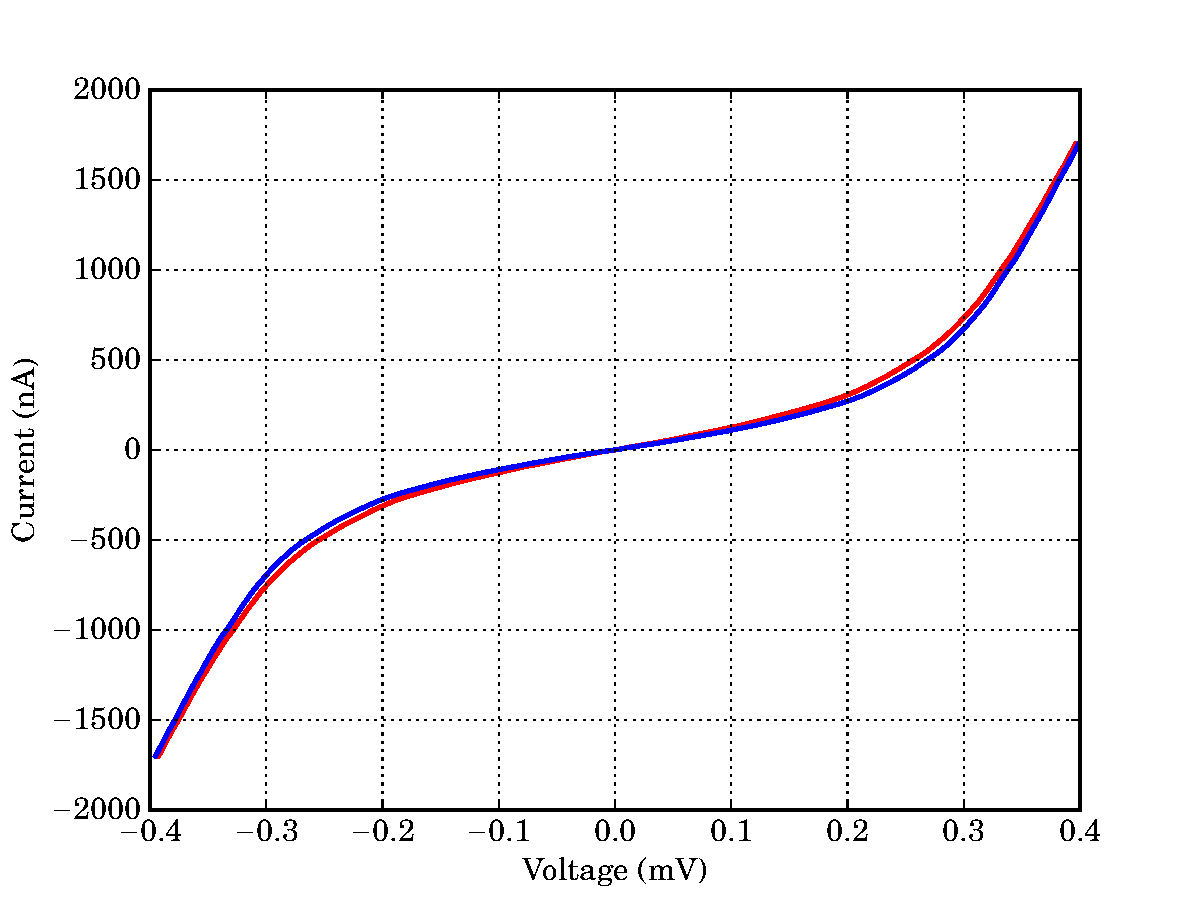
\includegraphics[width = 0.95\textwidth]{figures/control_IVs_77_300}
\caption[Current-voltage measurements for an optically-loaded unstrained SiCEB]{Current-voltage measurements for the unstrained detector. \gls{acr:IV} curves were recorded with the detector \textit{looking} at a 77-Kelvin source (blue) and a room-temperature source (red). Both measurements were made at a bath temperature of $350~\mathrm{mK}$.}
\label{fig:controlIVs_optical}
\end{center}
\end{figure}
\par 
The results of these measurements are shown in Figure~\ref{fig:controlIVs_optical}. Firstly, it is clear from this figure that these measurements did not suffer from the contamination which affected those presented in Figure~\ref{fig:controlIVs}. More significantly, however, Figure~\ref{fig:controlIVs_optical} shows that there is a measurable difference in the current-voltage characteristics for the two sources. The \gls{acr:IV} measurement taken with the lower-power source (the blue curve in Figure~\ref{fig:controlIVs_optical}) sits outside the measurement made with the higher-power source (red curve). The additional power from the room-temperature source causes the \gls{acr:IV} curve to shift towards the linear, in a similar way to increasing the bath temperature in the dark measurements (see Figure~\ref{fig:controlIVs}). This clearly makes sense, as in both scenarios, the energy of the carriers within the absorber was increased. It should, however, be noted that increasing the carrier energy via the optical system is much more efficient, since power is coupled to the carriers directly, as opposed to when the bath temperature increases, where power must flow through the weak thermal link between the electron and phonon systems. In both the cases shown in Figure~\ref{fig:controlIVs_optical}, the \gls{acr:IV} curve has substantially shifted towards the linear when compared to the $350~\mathrm{mK}$ curve shown in Figure~\ref{fig:controlIVs}.
\par 
Using Equation~\ref{res:IV}, it was possible to calculate the electron temperature (as was performed for the dark measurements). The results of this electron-temperature fitting are shown in Figure~\ref{fig:controlTe_optical}.
\begin{figure}[tb]
\begin{center}
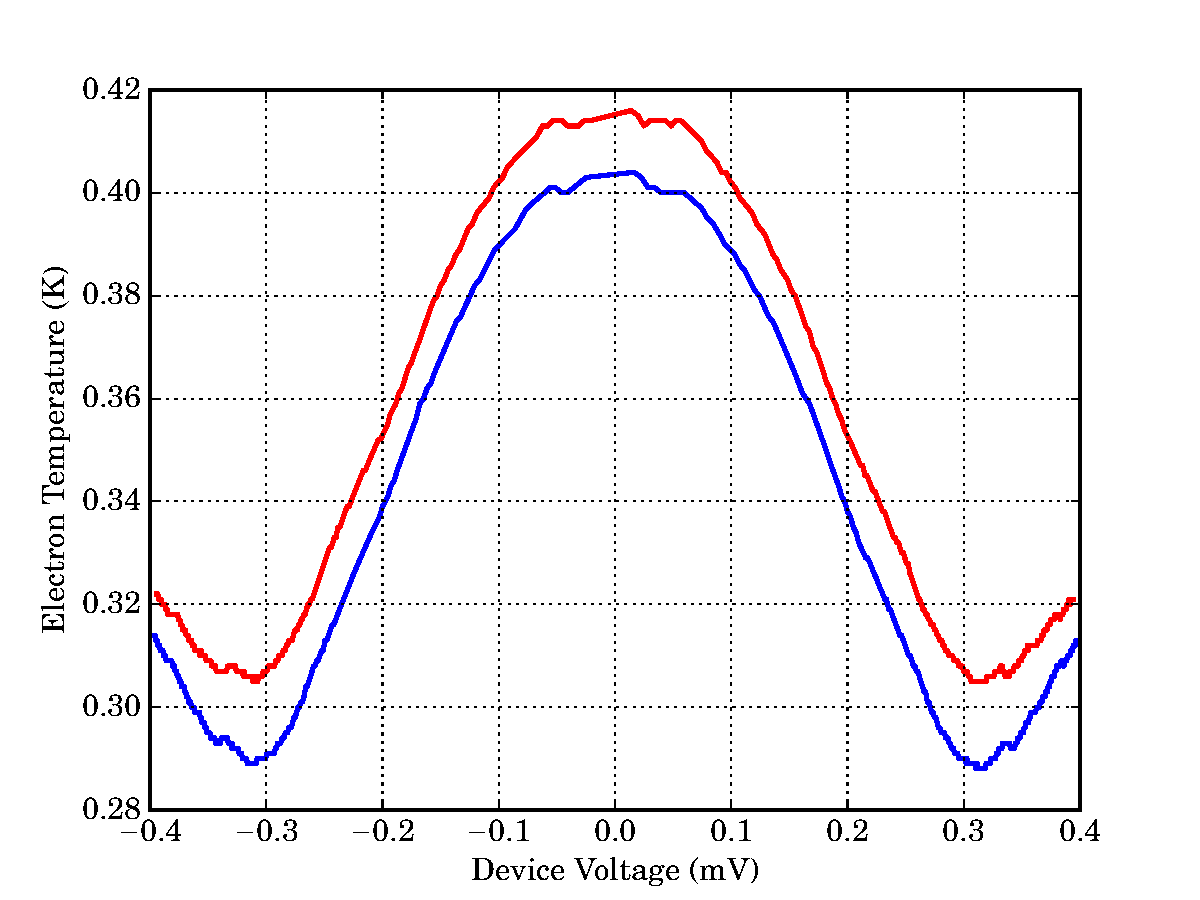
\includegraphics[width = 0.95\textwidth]{figures/control_Te_77_300}
\caption[Electron temperature for an optically-loaded unstrained \gls{acr:SiCEB}]{Electron-temperature fitting for the unstrained detector. This has been computed from the two optically-loaded \gls{acr:IV} curves shown in Figure~\ref{fig:controlIVs_optical}. The two curves correspond to the different optical sources. Blue---77-Kelvin source; red---room-temperature source. Note that, due to the optical load in these measurements, $T_{\mathrm{e}}$ at $V = 0$ is not equal to $T_{\mathrm{ph}}$. Measured at $350~\mathrm{mK}$.}
\label{fig:controlTe_optical}
\end{center}
\end{figure}
\begin{table}[htb]
\caption[Parameters used in electron-temperature fitting of unstrained-silicon detector with optical loading]{Parameters used in electron-temperature fitting of unstrained-silicon detector with optical loading.} 
\label{tab:ControlTeParams_optical}
\centering
\begin{tabular}{cccccc}
\toprule\toprule
$R_{\mathrm{abs}}$ & $2R_{\mathrm{N}}$ & $V_{\mathrm{J}}$ & $\varDelta$ & $\varDelta_{T=0}$ & $T_{\mathrm{c}}$ \\ \midrule
$50~\mathrm{\Omega}$ & $60~\mathrm{\Omega}$ & $V_{\mathrm{dev}} - IR_{\mathrm{abs}}$ 
& BCS, $\varDelta\left(T_{\mathrm{e}},~T_{\mathrm{c}}\right)$ & $160~\mathrm{\upmu eV}$ & $1.05~\mathrm{K}$ \\
\bottomrule
\end{tabular}
\end{table}
\par 
Electron-temperature fitting was performed using the parameters shown in Table~\ref{tab:ControlTeParams_optical}. Figure~\ref{fig:controlTe_optical} shows that the electron temperature has been raised substantially from the bath temperature of $350~\mathrm{mK}$. For the 77-Kelvin source, the electrons have been raised to $400~\mathrm{mK}$ at zero bias, whereas for the higher-power source (room-temperature source), the electrons are warmed to $415~\mathrm{mK}$ in the absence of any bias. This rise in the carrier temperature is entirely due to the optical power and is limited by the thermal link (described in Section~\ref{sec:eph}) to the lattice, which remains at the bath termpature of $350~\mathrm{mK}$. Electron cooling can still be seen in Figure~\ref{fig:controlTe_optical}, with the minimum achieved electron temperature being $290$ and $310~\mathrm{mK}$ for the 77-Kelvin and room-temperature sources respectively.
\par 
By noting that, in the absence of any bias, Equation~\ref{eqn:heatBalance} can be rewritten as:
\begin{align}
P + P_{\mathrm{abs}} + P_{\mathrm{J}} - P_{\mathrm{e\mbox{-}ph}} &= 0\,, \tag{Equation~\ref{eqn:heatBalance} revisited}\\
P_{\mathrm{abs}} &= P_{\mathrm{e\mbox{-}ph}}\,, \label{eqn:Pabs_V0}
\end{align}
it is possible to calculate the power absorbed within the detector by using Equation~\ref{def:e-phPower}. Doing so gave the absorbed power to be $34~\mathrm{pW}$ for the 77-Kelvin source and $43~\mathrm{pW}$ for the room-temperature source.
%
\subsection{Responsivity}\label{ssec:opticalControlSi_responsivity}
Given the electron temperature (found above), combined with the physical parameters of the detector, it is possible to calculate the responsivity of the detector using Equation~\ref{res:Vresponsivity}. This is expected to be different for the two different levels of optical loading, since the tunnelling current (and thus the voltage) is not linearly dependant on the electron temperature (see Figure~\ref{fig:IvsTe_model} for example). This analysis has been performed and the results are shown in Figure~\ref{fig:controlResponsivity}. In this figure, the absolute value of the responsivity has been plotted since, in a current-biased regime, the responsivity has the opposite sign to that of the bias (i.e. additional incident power always causes the measured voltage to shift towards zero).
\begin{figure}[tb]
\begin{center}
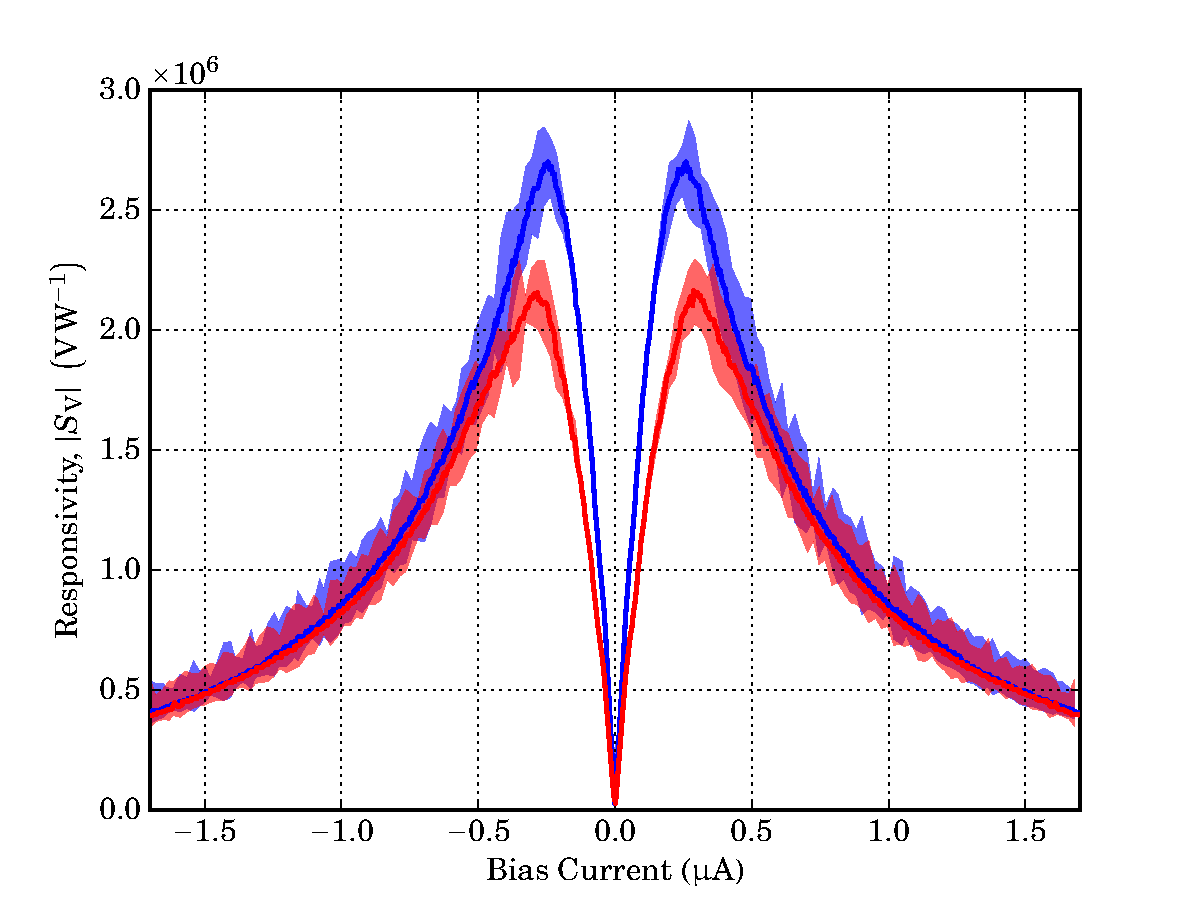
\includegraphics[width = 0.95\textwidth]{figures/control_responsivity}
\caption[Responsivity of an unstrained-\gls{acr:SiCEB}]{Responsivity of an unstrained-silicon cold-electron bolometer. Blue---77-Kelvin Source; red---room-temperature source. Shaded regions---uncertainty in responsivity. Measured at $350~\mathrm{mK}$.}
\label{fig:controlResponsivity}
\end{center}
\end{figure}
\par 
From Figure~\ref{fig:controlResponsivity}, it can be seen that the maximum responsivity achieved for this detector was $2.7 \times 10^{6}~\mathrm{V\,W^{-1}}$ at a bias of $250~\mathrm{nA}$ for the case where the detector was illuminated with a 77-Kelvin source. For the room-temperature source, the maximum responsivity was $2.1 \times 10^{6}~\mathrm{V\,W^{-1}}$. In both cases, the peak responsivity occurs at the same optimum bias of $\sim \pm 250~\mathrm{nA}$. It is also worth noting that Equation~\ref{res:Vresponsivity} does not depend on a measured optical power.
\par 
The error in the responsivity is governed by two main sources. Firstly, the error in the bias current across the device, which, more accurately, is the error in the current calculated for the electron temperature fitting described in Section~\ref{ssec:opticalControlSi_IV} and the error in the electron temperature itself. The total error in a measurement is given by the well-known equation:
\begin{align}
\left(\Delta Z\right)^{2} = 
	\left(\frac{\partial Z}{\partial x}\right)^{2}\left(\Delta x\right)^{2} + 
	\left(\frac{\partial Z}{\partial y}\right)^{2}\left(\Delta y\right)^{2} +
	\dots \,, \label{eqn:Error}
\end{align}
where $Z$ is the final quantity, $x$ and $y$ are measurements used to obtain $Z$, and $\Delta x$ and $\Delta y$ are their respective uncertainties. Applying this to the situation presented here, we find that the error in the detectors' responsivity is given by:
\begin{align}
\left(\Delta S_{\mathrm{V}}\right)^{2} = 
	\left(\frac{\partial S_{\mathrm{V}}}{\partial I}\right)^{2}
		\left(\Delta I\right)^{2} +
	\left(\frac{\partial S_{\mathrm{V}}}{\partial T_{\mathrm{e}}}\right)^{2}
		\left(\Delta T_{\mathrm{e}}\right)^{2}\,. \label{eqn:errorSv}
\end{align}
To calculate $\Delta S_{\mathrm{V}}$, the differentials have been calculated programmatically in a Python script, $\Delta I$ has been taken from the error in the current-fitting script utilised in Section~\ref{ssec:opticalControlSi_IV} (which is automatically calculated), and $\Delta T_{\mathrm{e}}$ has been taken to be $0.005~\mathrm{K}$ which is due to the electron temperature fitting resolution. The results of this error calculation are shown as the shaded regions in Figure~\ref{fig:controlResponsivity}. This shows that at peak responsivity, the uncertainty is $\pm 1.5 \times 10^{6}~\mathrm{V\,W^{-1}}$ when observing the 77-Kelvin source and $\pm 1.3 \times 10^{6}~\mathrm{V\,W^{-1}}$ when observing the room-temperature source.\footnote{Note that while the uncertainty is close to symmetric at peak bias, this is not generally the case.}
%
\subsection{Noise Measurements}\label{ssec:opticalControlSi_noise}
The noise voltage of the unstrained detector has been measured using the cross-correlated noise-measurement technique described in Section~\ref{sec:cross_col_noise}. This has been performed for both of the sources described above at current biases around the peak response ($250~\mathrm{nA}$). Averaging was performed on 201 acquisitions, which resulted in a correlated-amplifier-noise level of $500~\mathrm{pV\,Hz^{\nicefrac{-1}{2}}}$ (as can be seen from Figure~\ref{fig:crossCol_NoiseSimData}). 
\par 
An example noise spectrum (in this case measured at optimum bias with the 77-Kelvin source) is shown in Figure~\ref{fig:controlNoisePlot77}. It can be seen that there is very little $\nicefrac{1}{f}$ noise present in this measurement and that the white-noise level is well established for frequencies of $10~\mathrm{Hz}$ and above. There is some $50\mbox{-}\mathrm{Hz}$ noise present in the measurement; however, harmonics of this are not seen above $300~\mathrm{Hz}$, after which, the spectrum is flat. This measurement was performed at a sampling rate of $200,000~\mathrm{samples~per~second}$ with $200,000~\mathrm{samples}$ per acquisition. These settings resulted in a Nyquist frequency of $100,000~\mathrm{Hz}$ and the roll-off due to the data acquisition system has been removed from Figure~\ref{fig:controlNoisePlot77}.
\begin{figure}[tb]
\begin{center}
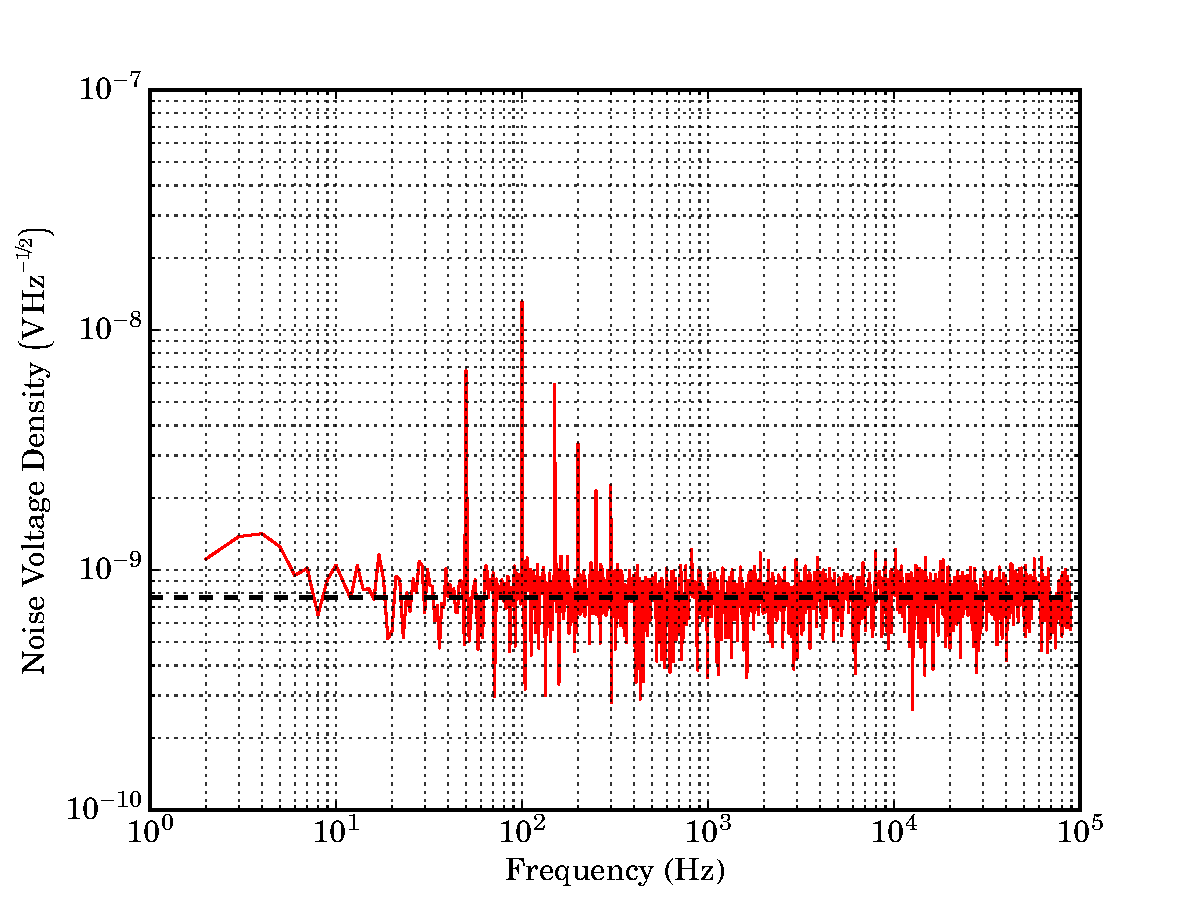
\includegraphics[width = 0.95\textwidth]{figures/control_noisePlot77}
\caption[Noise spectrum, measured at optimum bias, for the unstrained \gls{acr:SiCEB}]{Noise spectral density, measured at optimum bias ($250~\mathrm{nA}$), for the unstrained \gls{acr:SiCEB}. Red---Noise spectrum; dashed line---average noise level across the entire spectrum. Data have been reduced via logarithmic binning to improve the clarity of the figure. Measured at $350~\mathrm{mK}$.}
\label{fig:controlNoisePlot77}
\end{center}
\end{figure}
\par 
The average noise levels from the measurements made at different bias levels and for the two optical sources has been collated and is shown in
Figure~\ref{fig:controlNoiseV}.
\begin{figure}[tb]
\begin{center}
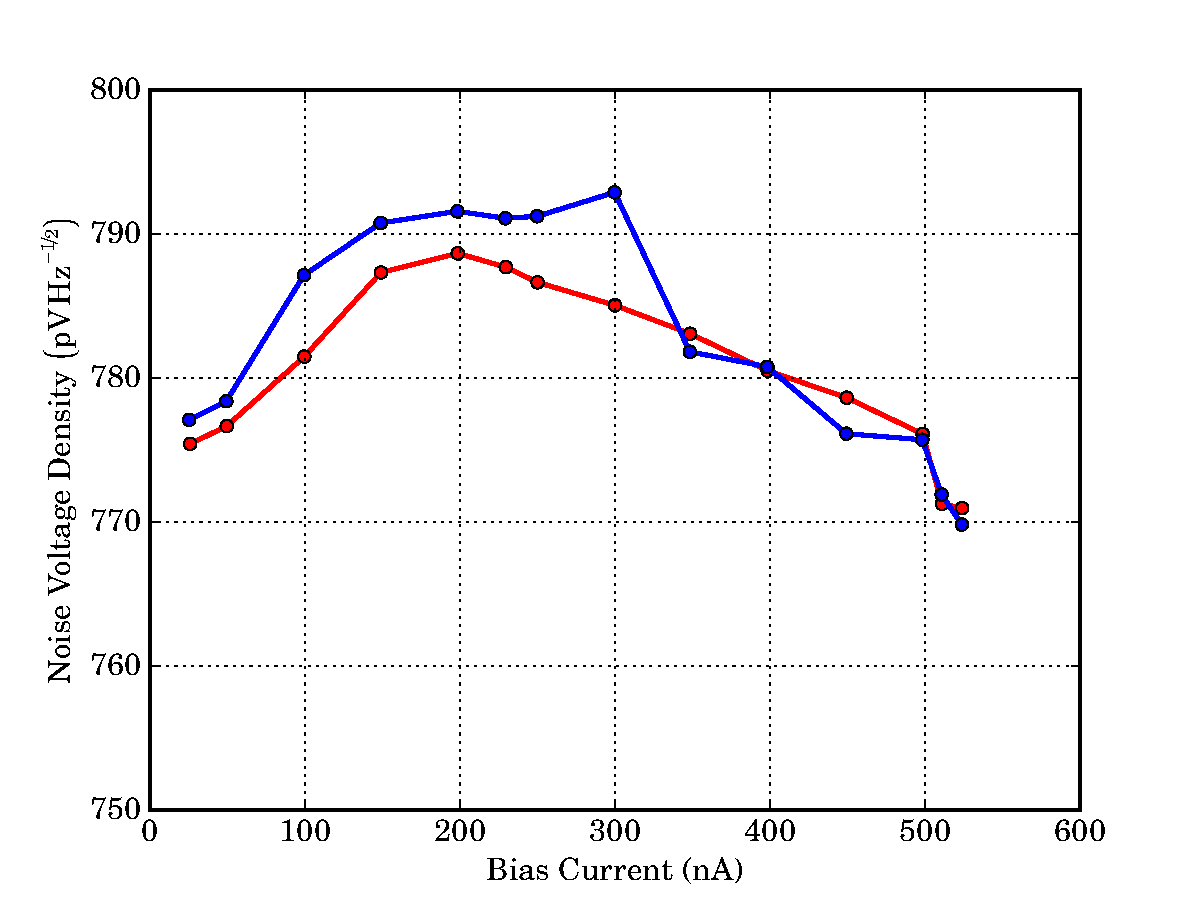
\includegraphics[width = 0.95\textwidth]{figures/control_noiseVoltage}
\caption[Summary of the change in noise voltage with bias current for the unstrained \gls{acr:SiCEB}]{Summary of the change in noise voltage with bias current for the unstrained \gls{acr:SiCEB}. Blue---77-Kelvin Source; red---room-temperature source. Measured at $350~\mathrm{mK}$.}
\label{fig:controlNoiseV}
\end{center}
\end{figure}
\par 
Figure~\ref{fig:controlNoiseV} shows that the unstrained detector has similar noise properties under both optical loadings. At optimum bias, the noise voltage measured when viewing the 77-Kelvin source is marginally ($6~\mathrm{pV\,Hz^{\nicefrac{-1}{2}}}$) higher than when viewing the room-temperature source; away from the optimum bias, the measured noise voltages are near-identical for the two different sources.
\par 
The noise-equivalent power of the detector in these situations can be found by dividing the measured noise voltage by the detectors responsivity and is shown (calculated from the various data above) in Figure~\ref{fig:controlNoiseNEP}. This figure shows that the noise-equivalent power is not dominated by the small differences seen in the noise voltage (Figure~\ref{fig:controlNoiseV}) but is dominated by the differences in the responsivity seen in Figure~\ref{fig:controlResponsivity}. The minimum achieved noise-equivalent power for the 77-Kelvin source was $2.9 \times 10^{-16}~\mathrm{W\,Hz^{\nicefrac{-1}{2}}}$, whereas for the room-temperature source, the minimum noise-equivalent power was marginally larger at $3.7 \times 10^{-16}~\mathrm{W\,Hz^{\nicefrac{-1}{2}}}$. This makes sense given the slightly larger responsivity found when the detector was illuminated by the 77-Kelvin source and noting that, in the case where the noise of the detector is hardly changing, $NEP \propto \nicefrac{1}{S}$.
\begin{figure}[tb]
\begin{center}
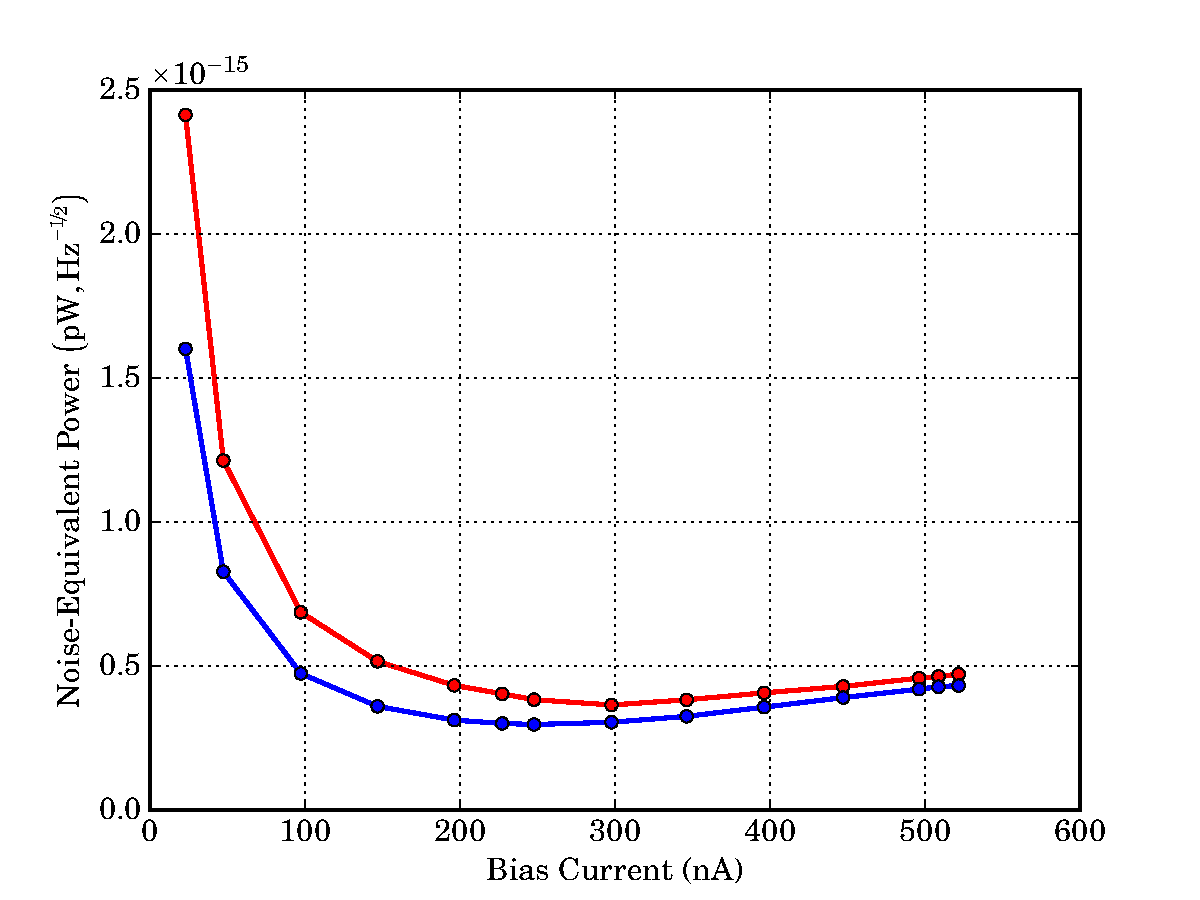
\includegraphics[width = 0.95\textwidth]{figures/control_NEP_77_300}
\caption[Noise-equivalent power of an unstrained-\gls{acr:SiCEB} biased at various currents around the optimum bias]{Noise-equivalent power of an unstrained-\gls{acr:SiCEB} biased at various currents around the optimum bias. Blue---77-Kelvin source; red---room-temperature source. Measured at $350~\mathrm{mK}$.}
\label{fig:controlNoiseNEP}
\end{center}
\end{figure}
\par 
The noise-equivalent power can be examined in a more complete fashion by using Equation~\ref{res:NEP_CEB}, combined with the results found previously in this chapter, to calculate the predicted contribution of the various noise sources to the total noise-equivalent power. The results of this noise modelling, for the case where the detector was illuminated by a room-temperature source, are presented in Figure~\ref{fig:controlNoiseModel300}. From this figure, it can be seen that, despite cross-correlation of the noise, the noise-equivalent power of the this device is mainly dominated by the amplifier noise; however, at the minimum value of the noise-equivalent power, the contribution from photon noise is discernible. The domination of the amplifier noise over the photon noise is due to the low responsivity of the detector---the responsivity decreases the amplifier noise as $S_{\mathrm{V}}^{-1}$, whereas the photon noise does not depend on the responsivity. The previously calculated \gls{acr:NEP} data show reasonable agreement with the model within their errors (discussed in the following paragraph). In the absence of any amplifier noise, the detector would have been photon-noise limited. Finally, if the photon noise is also disregarded, the device-limited noise-equivalent power (given by the combination of the tunnelling noise and the electron-phonon heat-flow noise) would have had a minimum value (shown by the dashed-black curve in Figure~\ref{fig:controlNoiseModel300}) of $4.8 \times 10^{-17}~\mathrm{W\,Hz^{\nicefrac{-1}{2}}}$.
\begin{figure}[tb]
\begin{center}
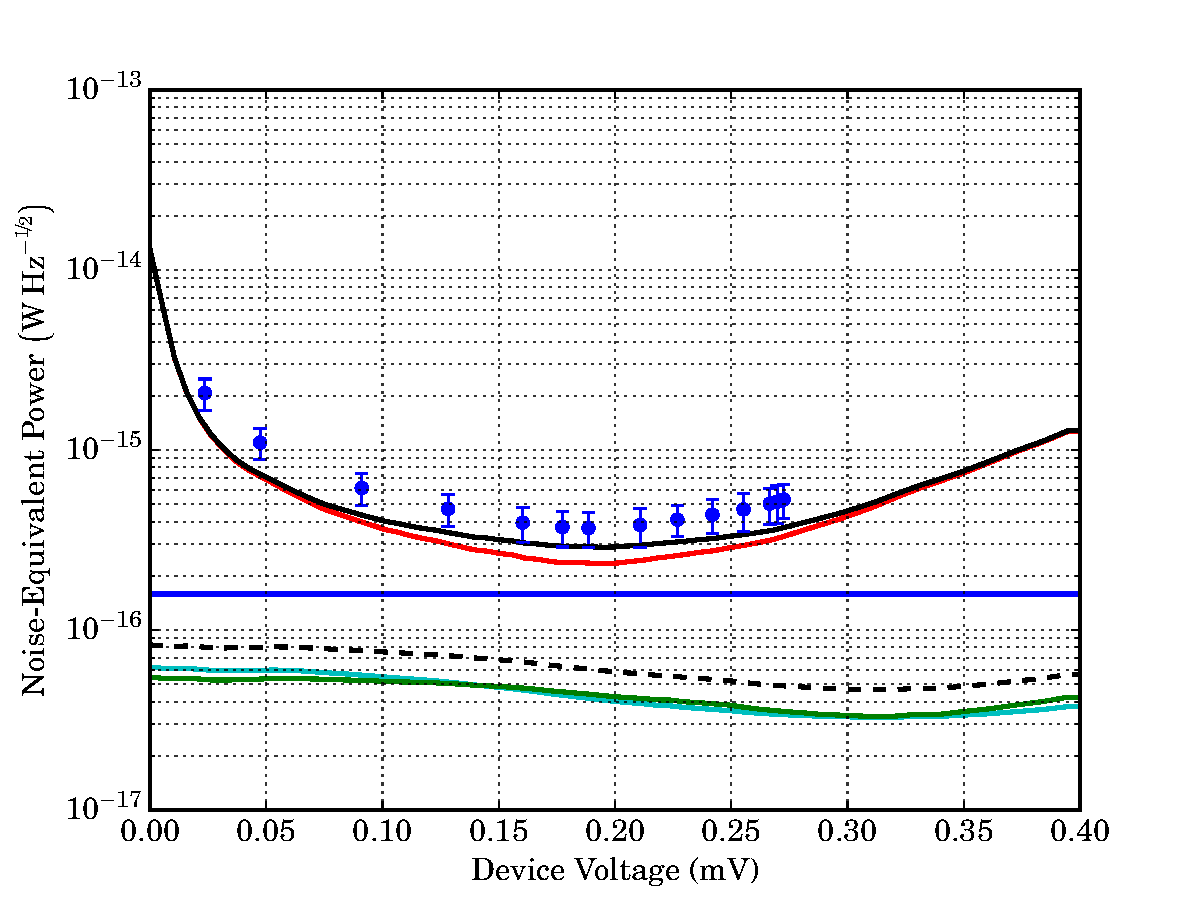
\includegraphics[width = 0.95\textwidth]{figures/control_noiseModel300}
\caption[Noise modelling for the unstrained-\gls{acr:SiCEB} observing a room-temperature source]{Noise modelling for the unstrained-\gls{acr:SiCEB} observing a room-temperature source. Cyan---Electron-phonon heat-flow noise; green---tunnelling noise, a combination of tunnelling-current noise and the tunnelling-heat-flow noise; blue---photon noise; red---amplifier noise; black (solid)---total noise; black (dashed)---total device noise; circles---data. Measured and calculated at $350~\mathrm{mK}$.}
\label{fig:controlNoiseModel300}
\end{center}
\end{figure}
\par 
The uncertainty in the noise-equivalent power (shown as the error bars on the data points in Figure~\ref{fig:controlNoiseModel300}) is given by:
\begin{align}
\left(\Delta\NEP\right)^{2} = 
	\left(\frac{\partial\NEP}{\partial S_{\mathrm{V}}}\right)^{2}
		\left(\Delta S_{\mathrm{V}}\right)^{2} + 
	\left(\frac{\partial\NEP}{\partial e_{\mathrm{tot}}}\right)^{2}
		\left(\Delta e_{\mathrm{tot}}\right)^{2}\,, \label{eqn:errorNEP}
\end{align}
where  $\Delta S_{\mathrm{V}}$ is the uncertainty in the voltage responsivity, given by Equation~\ref{eqn:errorSv}, and $e_{\mathrm{tot}}$ is the noise spectral density measured at the oscilloscope. Since the white noise is Gaussian, we can write:
\begin{align}
\Delta e_{\mathrm{tot}} = \sigma\left(e_{\mathrm{tot}}\right)\,.
\end{align}
This means that Equation~\ref{eqn:errorNEP} can be written as:
\begin{align}
\left(\Delta\NEP\right)^{2} = 
	\left(\frac{\partial\NEP}{\partial S_{\mathrm{V}}}\right)^{2}
		\left(\Delta S_{\mathrm{V}}\right)^{2} + 
	\left(\frac{\partial\NEP}{\partial e_{\mathrm{tot}}}\right)^{2}
		\left(\sigma\left(e_{\mathrm{tot}}\right)\right)^{2}\,. 
\label{eqn:errorNEPsub}
\end{align}
Using Equation~\ref{def:NEP} for the noise-equivalent power, the uncertainty is given by:
\begin{align}
\left(\Delta\NEP\right)^{2} =
	\left(\frac{1}{S_{\mathrm{V}}}\right)^{2}
		\left(\Delta S_{\mathrm{V}}\right)^{2} +
	\left(\frac{-e_{\mathrm{tot}}}{S_{\mathrm{V}}^{2}}\right)^{2}
		\left(\sigma e_{\mathrm{tot}}\right)^{2}\,. \label{eqn:errorNEPfinal}
\end{align}
Examining the contributions of this for the minimum noise-equivalent power shown in Figure~\ref{fig:controlNoiseModel300} ($3.7 \times 10^{-16}~\mathrm{W\,Hz^{\nicefrac{-1}{2}}}$) shows that the uncertainty in $\NEP$ due to the responsivity is $^{+5.1}_{-4.7}\times 10^{-18}~\mathrm{W\,Hz^{\nicefrac{-1}{2}}}$,\footnote{Note this error is asymmetric for the reasons discussed in Section~\ref{ssec:opticalControlSi_responsivity}.} whereas the error due to measurement of the noise spectrum was $\pm 7.8 \times 10^{-17}~\mathrm{W\,Hz^{\nicefrac{-1}{2}}}$. From this, it is clear that the total error is dominated by the error associated with the measurement of the noise spectrum.
\par 
\begin{figure}[tb]
\begin{center}
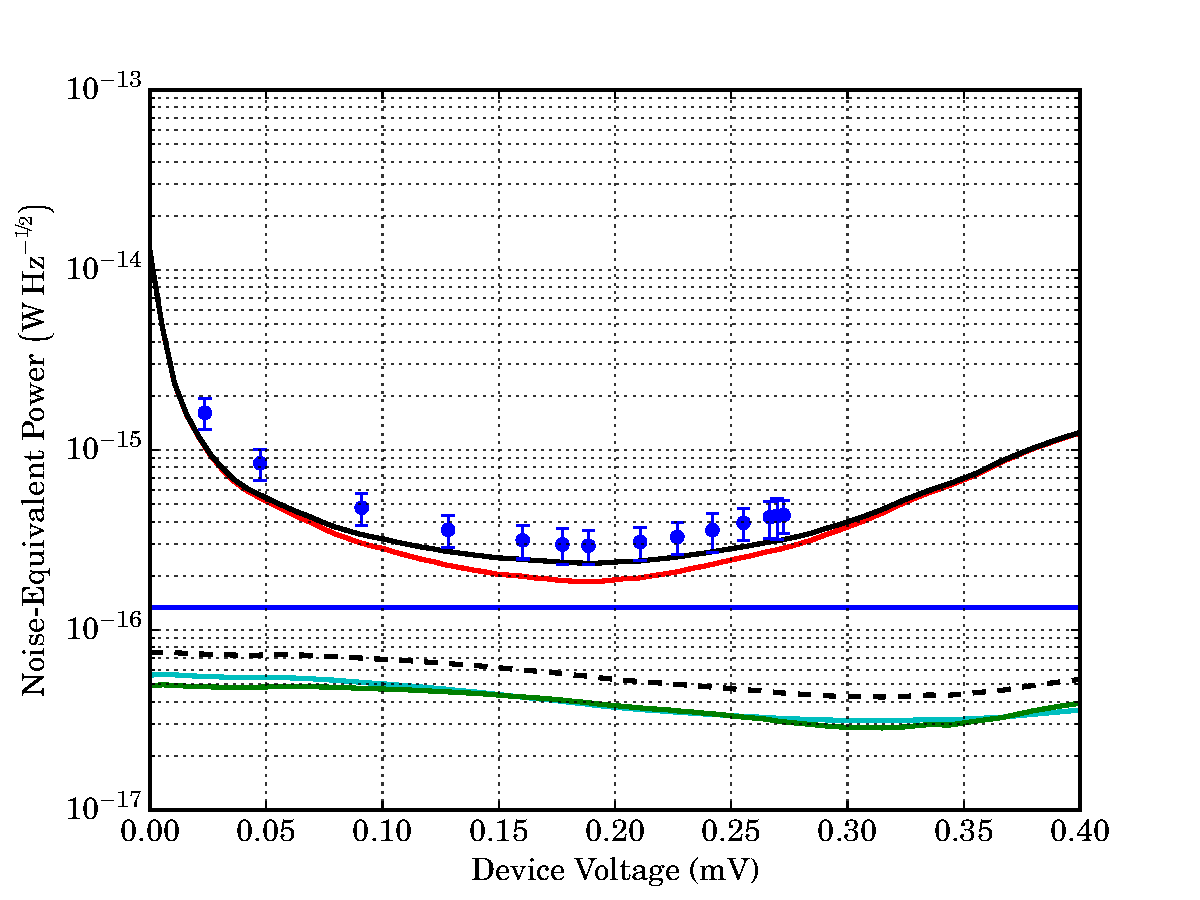
\includegraphics[width = 0.95\textwidth]{figures/control_noiseModel77}
\caption[Noise modelling for the unstrained-\gls{acr:SiCEB} observing a 77-Kelvin source]{Noise modelling for the unstrained-\gls{acr:SiCEB} observing a 77-Kelvin source. Cyan---Electron-phonon heat-flow noise; green---tunnelling noise, a combination of tunnelling-current noise and the tunnelling-heat-flow noise; blue---photon noise; red---amplifier noise; black (solid)---total noise; black (dashed)---total device noise; circles---data. Measured and calculated at $350~\mathrm{mK}$.}
\label{fig:controlNoiseModel77}
\end{center}
\end{figure}
Repeating the above analysis for the case where the detector was illuminated by a 77-Kelvin source yields similar results with the noise-equivalent power being dominated by the amplifier noise, although, again, the contribution from the photon noise can be observed at optimum bias. The minimum achieved noise-equivalent power in this case was $2.4 \times 10^{-16}~\mathrm{W\,Hz^{\nicefrac{-1}{2}}}$ and the minimum device noise limited noise-equivalent power was $4.2 \times 10^{-17}~\mathrm{W\,Hz^{\nicefrac{-1}{2}}}$. These results are shown in Figure~\ref{fig:controlNoiseModel77}.
%
\subsection{Spectral Response}\label{ssec:opticalControlSi_spectral}
\begin{figure}[tb]
\begin{center}
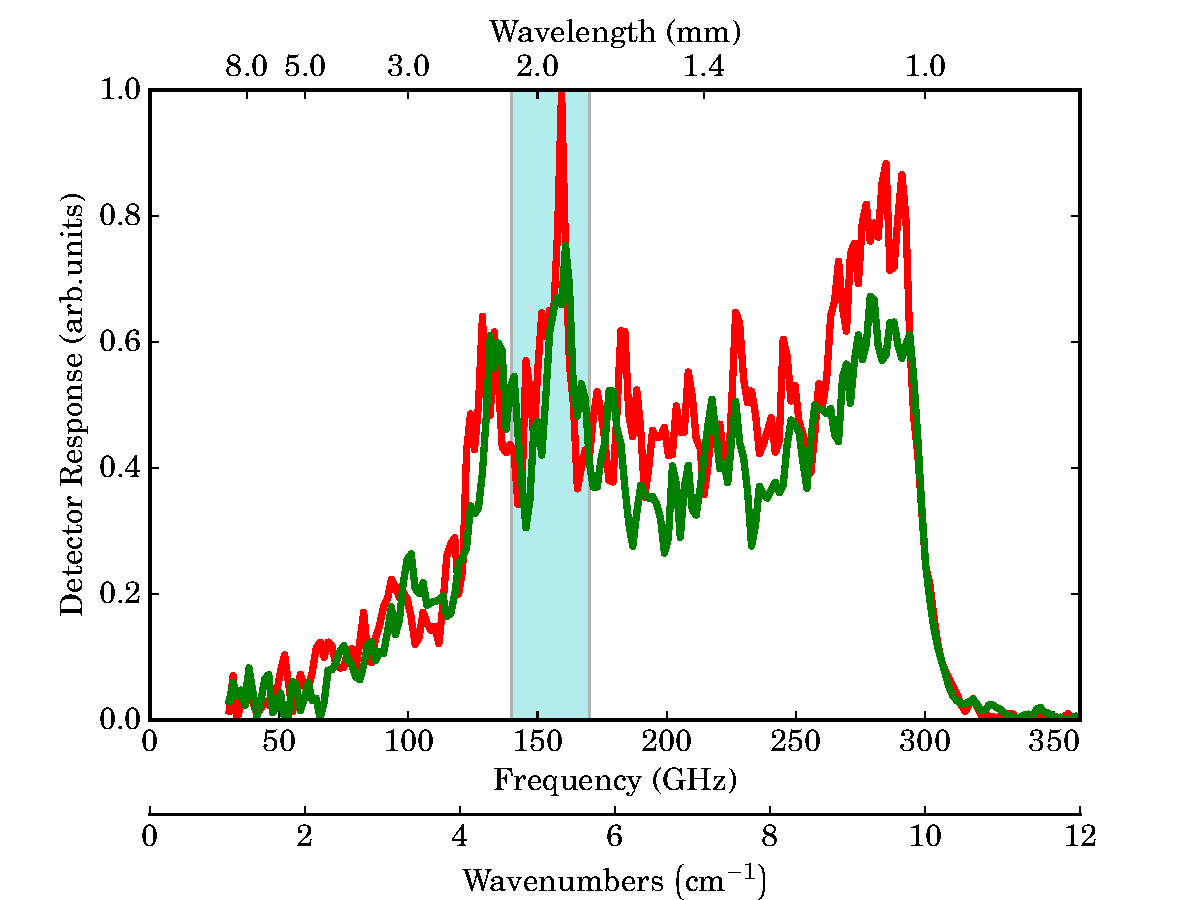
\includegraphics[width = 0.95\textwidth]{figures/control_FTS}
\caption[Spectral response of the control-SiCEB]{Spectral response of the unstrained-\gls{acr:SiCEB}, measured using a Fourier-transform spectrometer. Red---polarisation vector aligned with antenna polarisation; green---polarisation vector perpendicular to antenna polarisation; highlighted region---expected region of antenna response. In these measurements, a mercury arc lamp was used as the source. Measured at $350~\mathrm{mK}$.}
\label{fig:controlSpectrum}
\end{center}
\end{figure}
The spectral response of the unstrained detector has been measured using Fourier transform spectrometer. This measurement was performed for both linear polarisations and the results are shown in Figure~\ref{fig:controlSpectrum}. When the polarisation of the spectrometer's source (a mercury arc lamp with a linear slot polarising grid) was aligned with that of the antenna (red line in Figure~\ref{fig:controlSpectrum}), a notable response is seen at the anticipated frequencies (shaded region in Figure~\ref{fig:controlSpectrum}). Where the source polarisation was rotated such to be orthogonal to that of the antenna (green line in Figure~\ref{fig:controlSpectrum}), this response was diminished. The overall plateau level seen in Figure~\ref{fig:controlSpectrum} is most likely due to direct, bolometric, absorption of radiation in the absorber or by the aluminium being slightly lossy and absorbing the radiation. Other features seen in the spectrum can most likely be attributed to reflections from the lens and within the device holder, since none of these surfaces were anti-reflection coated. These issues are explored to greater detail in Section~\ref{sec:antennaSims}. The loss of detector response at $300~\mathrm{GHz}$ is simply the result of the low-pass filter used in this measurement. 
%
\section{Strained Silicon}\label{sec:opticalStrainedSi}
All the characterisation work detailed in the previous section for the unstrained detector has been replicated for the detector with a strained-silicon absorber (previously covered in Section~\ref{sec:darkControlSi}). The experimental conditions were replicated as closely as possible between the two experiments; with one exception being that the optical configuration was slightly different, in that the back-to-back horn pair were placed slightly further away from the detector, slightly reducing the optical throughput of the optics system. Further to these tests, as mentioned in the introduction to this chapter, the response of this detector to a chopped source (an emitting-diode source tuned to output $150~\mathrm{GHz}$) has also been measured.
%
\subsection{Current-Voltage Measurements}\label{ssec:opticalStrainedSi_IV}
As was the case for the unstrained detector, \gls{acr:IV} curves have been measured with the detector illuminated by two different sources: room-temperature Eccosorb and Eccosorb cooled in liquid nitrogen to $77~\mathrm{K}$. As with the previous measurement for the unstrained device, the optical testing was carried out at a bath temperature of $350~\mathrm{mK}$. The results of these measurements can be seen in Figure~\ref{fig:strainedIVs_optical}. From this figure, it can be seen that the general behaviour is similar to the previously tested detector, in that the additional optical power causes the \gls{acr:IV} curve to tend towards the linear. When a closer comparison to the current-voltage characteristics of the unstrained detector (as shown in Figure~\ref{fig:controlIVs_optical}) is made, it is apparent that the response for this detector is noticeably larger (i.e. the \gls{acr:IV} curve for the room-temperature source is much more clearly distinguished from the curve for the 77-Kelvin source than was seen previously). This is even more impressive considering that, as discussed above, the incident optical power on this detector was expected to be lower than for the unstrained device, due to differences in the optical configuration.
\begin{figure}[tb]
\begin{center}
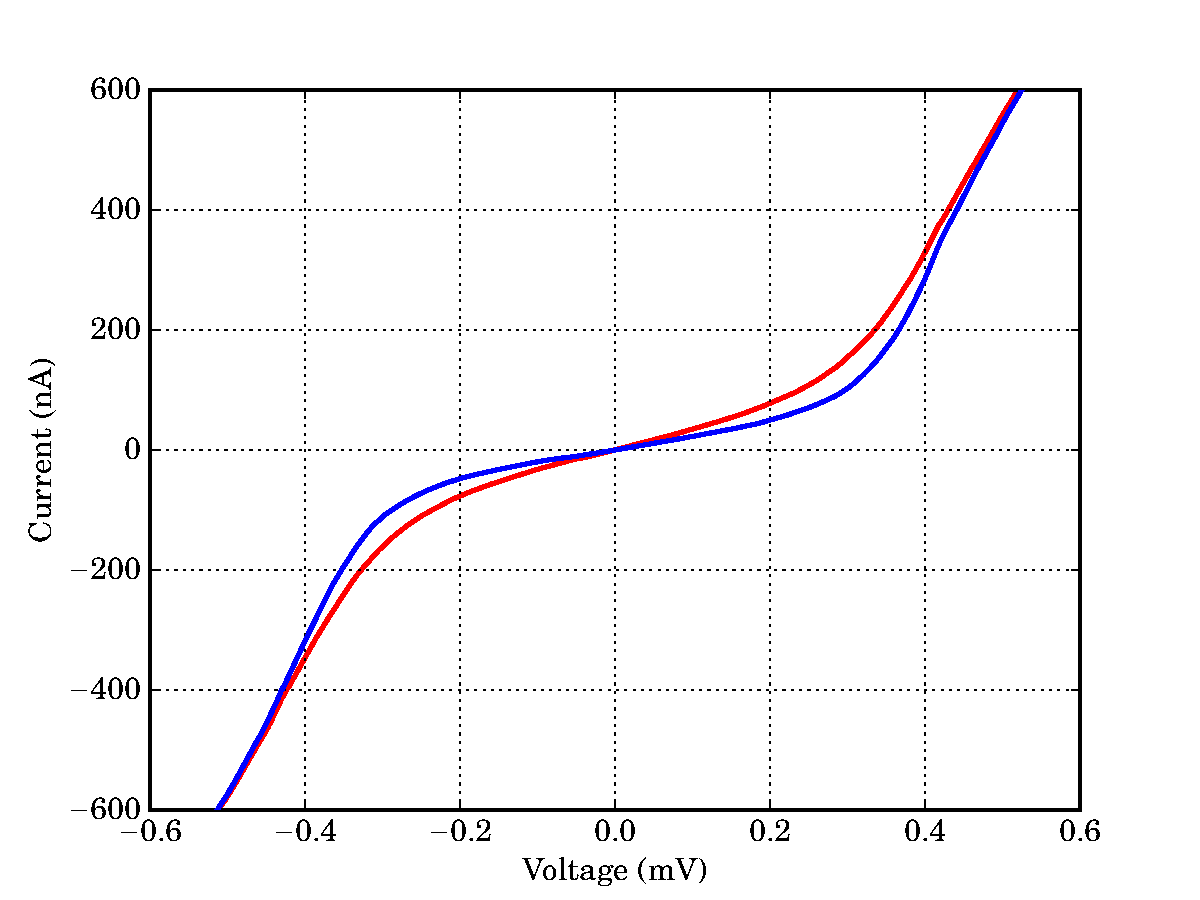
\includegraphics[width = 0.95\textwidth]{figures/strained_IVs_77_300}
\caption[Current-voltage measurements for an optically-loaded strained-\gls{acr:SiCEB}]{Current-voltage measurements for the strained detector. \gls{acr:IV} curves were recorded with the detector illuminated by both a 77-Kelvin source (blue) and a room-temperature source (red). Both measurements were made at a bath temperature of $350~\mathrm{mK}$.}
\label{fig:strainedIVs_optical}
\end{center}
\end{figure}
\par 
The overall characteristics of the \gls{acr:IV} curves seen in Figure~\ref{fig:strainedIVs_optical} are in line with those previously measured in the absence of any optical power (shown in Figure~\ref{fig:strainedIVs}). As has been performed for both sets of dark measurements and the optically loaded \gls{acr:IV} curves for the unstrained detector, the electron temperature has been calculated as a function of the voltage across the detector by fitting the \gls{acr:IV} curves to Equation~\ref{res:IV}. This is shown in Figure~\ref{fig:strainedTe_optical}. The electron temperature in the absence of any bias was calculated to be $550~\mathrm{mK}$ for the 77-Kelvin source and $630~\mathrm{mK}$ for the room-temperature source. These increases from the bath temperature of $350~\mathrm{mK}$ are greater than was seen for the unstrained detector (Figure~\ref{fig:controlTe_optical}); this is the result of the substantially reduced electron-phonon coupling in this sample ($2.0 \times 10^{7}~\mathrm{W\,K^{-6}\,m^{-3}}$), compared to the unstrained detector ($5.8 \times 10^{8}~\mathrm{W\,K^{-6}\,m^{-3}}$), as discussed in Section~\ref{sec:eph}. The parameters used in the electron-temperature fitting are given in Table~\ref{tab:strainedTeParams_optical}.
\begin{figure}[tb]
\begin{center}
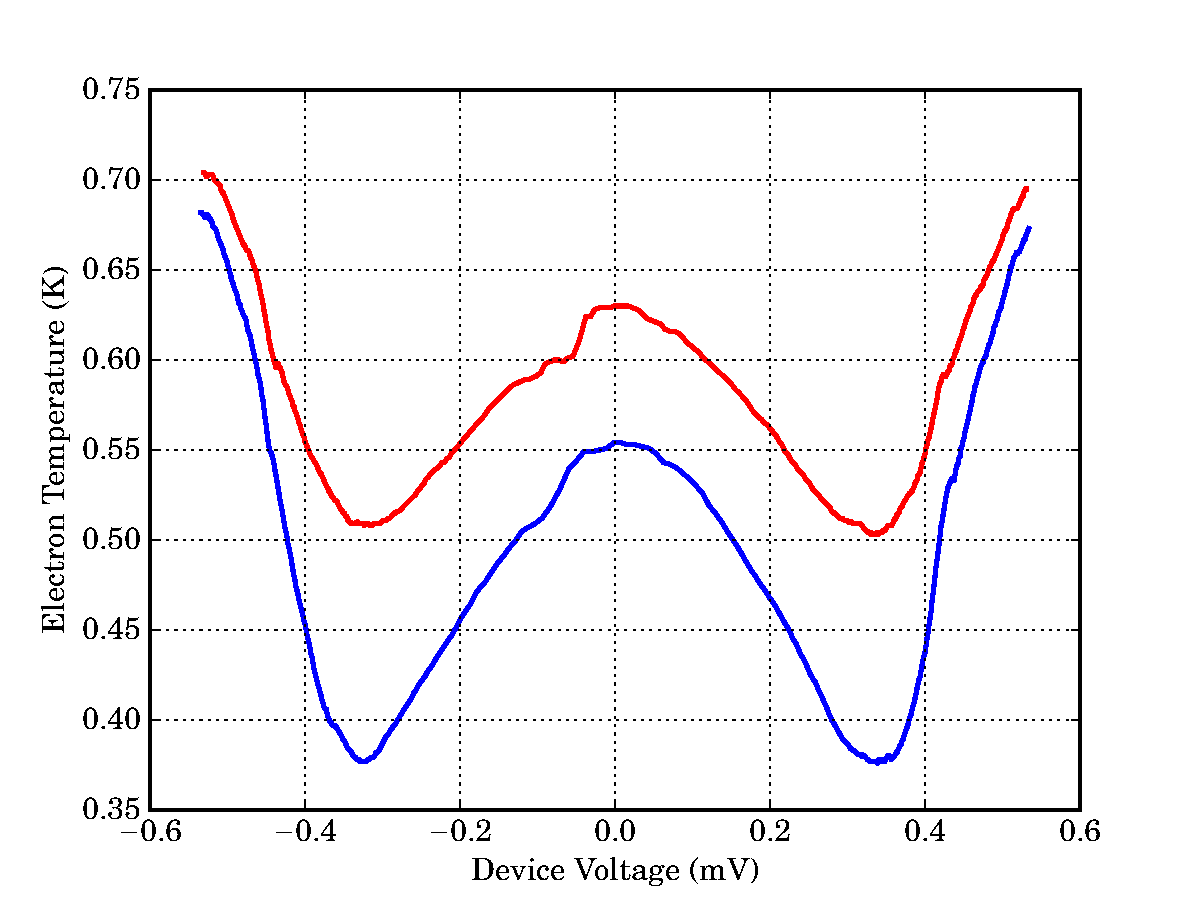
\includegraphics[width = 0.95\textwidth]{figures/strained_Te_77_300}
\caption[Electron temperature of strained-\gls{acr:SiCEB} under optical loading]{Electron temperature of strained-\gls{acr:SiCEB} under optical loading. Blue---77-Kelvin source; red---room-temperature source. Measured at a thermal bath temperature of $350~\mathrm{mK}$. Measured at $350~\mathrm{mK}$.}
\label{fig:strainedTe_optical}
\end{center}
\end{figure}
\begin{table}[htb]
\caption[Parameters used in electron-temperature fitting of strained-silicon detector with optical loading]{Parameters used in electron-temperature fitting of strained-silicon detector with optical loading.} 
\label{tab:strainedTeParams_optical}
\centering
\begin{tabular}{cccccc}
\toprule\toprule
$R_{\mathrm{abs}}$ & $2R_{\mathrm{N}}$ & $V_{\mathrm{J}}$ & $\varDelta$ & $\varDelta_{T=0}$ & $T_{\mathrm{c}}$ \\ \midrule
$75~\mathrm{\Omega}$ & $580~\mathrm{\Omega}$ & $V_{\mathrm{dev}} - IR_{\mathrm{abs}}$ 
& BCS, $\varDelta\left(T_{\mathrm{e}},~T_{\mathrm{c}}\right)$ & $182~\mathrm{\upmu eV}$ & $1.2~\mathrm{K}$ \\
\bottomrule
\end{tabular}
\end{table}
\par 
By using Equation~\ref{eqn:Pabs_V0}, the absorbed power in the detector for the two optical sources was found to be $9.2~\mathrm{pW}$ for the 77-Kelvin source and $20.0~\mathrm{pW}$ for the room-temperature source. These values support the assertion at the start of this section that the optical power would be reduced in these measurements compared to those performed for the unstrained detector, due to small changes in the optical setup.
%
\subsection{Responsivity}\label{ssec:opticalStrainedSi_responsivity}
The responsivity of the strained-silicon device has been found using Equation~\ref{res:Vresponsivity} and is shown in Figure~\ref{fig:strainedResponsivity}. The maximum responsivity occurred when the detector was illuminated by the 77-Kelvin source and had a peak value of $\left(1.5^{+0.5}_{-1.0}\right) \times 10^{7}~\mathrm{V\,W^{-1}}$. The maximum responsivity when the detector was illuminated by the room-temperature source was $\left(4.6 \pm 0.4\right) \times 10^{6}~\mathrm{V\,W^{-1}}$. The responsivity was slightly higher under negative biases, this was most likely the result of minor misalignment during the fabrication process, creating slightly asymmetric contacts to the absorber. The optimum bias for this detector was found to be $-90~\mathrm{nA}$ with $+90~\mathrm{nA}$ being the optimum current under positive bias. The uncertainty in these measurements has been calculated as discussed in Section~\ref{ssec:opticalControlSi_responsivity}.
\begin{figure}[tb]
\begin{center}
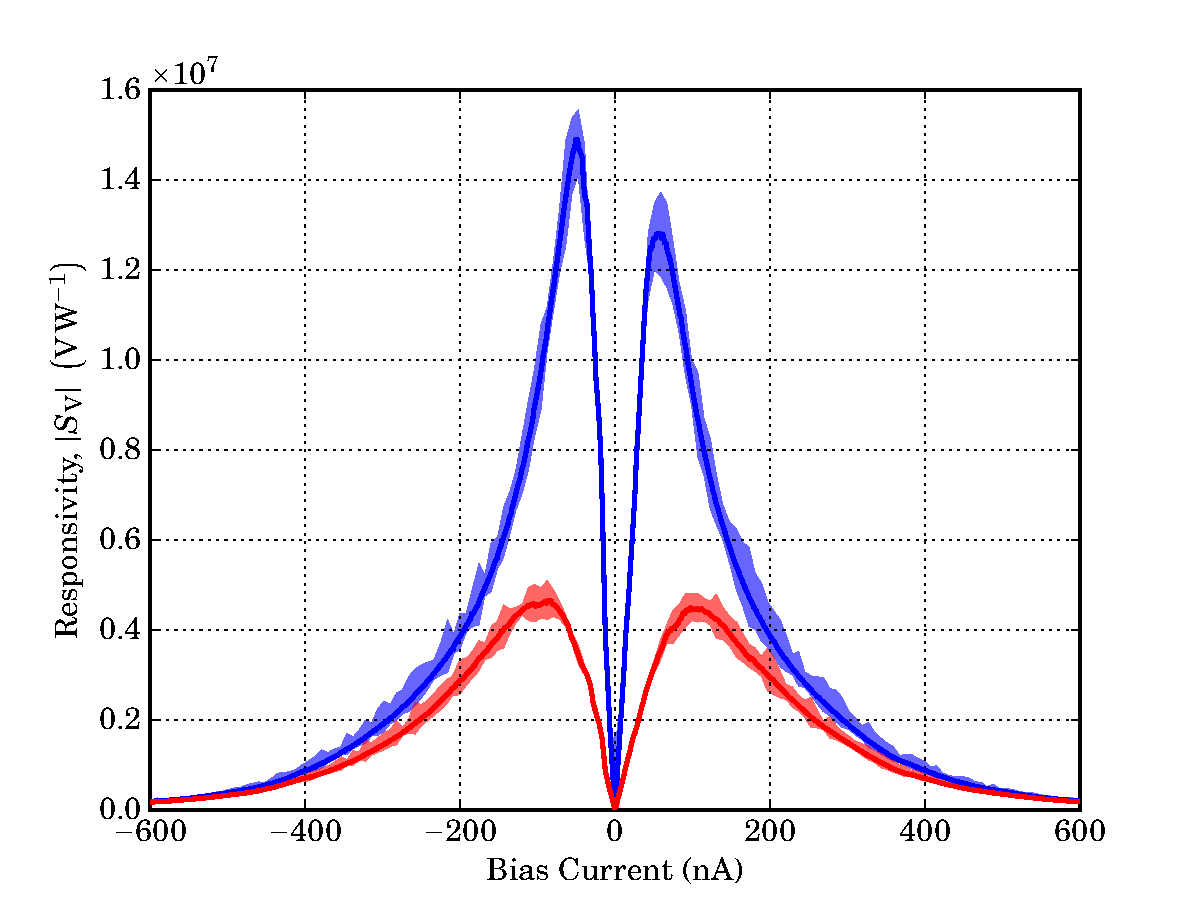
\includegraphics[width = 0.95\textwidth]{figures/strained_responsivity}
\caption[Responsivity of the strained-\gls{acr:SiCEB} device]{Responsivity of the strained-silicon cold-electron bolometer. Blue---77-Kelvin Source; red---room-temperature source. Shaded regions---uncertainty in responsivity. Measured at $350~\mathrm{mK}$.}
\label{fig:strainedResponsivity}
\end{center}
\end{figure}
\par 
It is interesting to note that the relative difference between the two curves shown in Figure~\ref{fig:strainedResponsivity} is greater than that seen in Figure~\ref{fig:controlResponsivity} for the unstrained detector, where the optical power was higher. This indicates that the responsivity is diminishing with increased optical loading. This can be seen in both Figures~\ref{fig:controlResponsivity} and \ref{fig:strainedResponsivity}, where, in both cases, the lower optical load (that from the 77-Kelvin source) has resulted in a higher responsivity. While this seems to makes sense when considering the unloaded current-voltage measurements (unstrained: Figure~\ref{fig:controlIVs}; strained: Figure~\ref{fig:strainedIVs}), where for higher bath temperatures the \gls{acr:IV} curves become increasingly linear and more closely packed, clearly further study---with a greater range of optical powers---is needed to fully explore this behaviour. The greater responsivity observed here is a clear indication that the reduced interaction between the electrons and phonons has resulted in a more responsive detector. This is, in part due to the fact that the absorber temperature in the strained sample is higher for an equivalent optical power compared to the unstrained detector; this again is a result of the reduced electron-phonon coupling, as described in Section~\ref{sec:eph}.
%
\subsection{Noise Measurements}\label{ssec:opticalStrainedSi_noise}
Electrical-noise spectra have been measured at a range of bias currents and with the detector illuminated by both the 77-Kelvin and the room-temperature source. These measurements were performed using the cross-correlated noise readout system used for the unstrained detector (that described in Section~\ref{sec:cross_col_noise}), with a similar number of averages being used in both scenarios.
\begin{figure}[tb]
\begin{center}
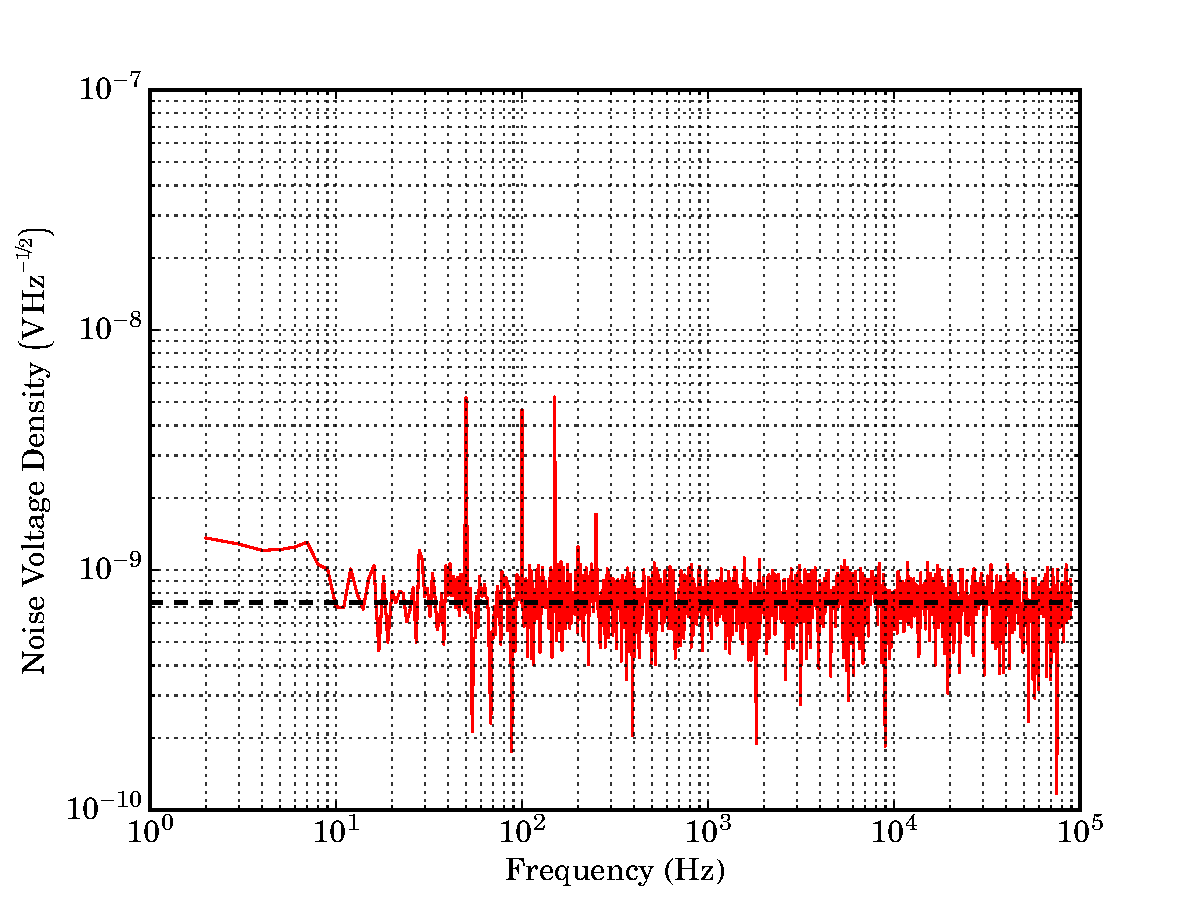
\includegraphics[width = 0.95\textwidth]{figures/strained_noisePlot77}
\caption[Noise spectrum for the strained-\gls{acr:SiCEB}]{Noise spectral density for the strained-\gls{acr:SiCEB}. This spectrum was measured away from the optimum bias (in terms of response), where the noise voltage was lowest and in the presence of a 77-Kelvin optical source. Red---Noise spectrum; dashed line---average noise level across the entire spectrum. Data have been reduced via logarithmic binning to improve the clarity of the figure. Measured at $350~\mathrm{mK}$.}
\label{fig:strainedNoisePlot77}
\end{center}
\end{figure}
\par 
Figure~\ref{fig:strainedNoisePlot77} shows a noise spectrum measured away from the optimum bias, where the noise voltage is lowest, for the strained detector. As was seen for the unstrained detector (Figure~\ref{fig:controlNoisePlot77}), the spectrum is almost entirely flat with a $\nicefrac{1}{f}$ component having diminished by $10~\mathrm{Hz}$ and little pickup. Limited 50-Hz pickup is seen from the mains supply but otherwise, there are few features in this spectrum. The roll-off due to the data acquisition system has been removed from the spectrum.
\par 
\begin{figure}[tb]
\begin{center}
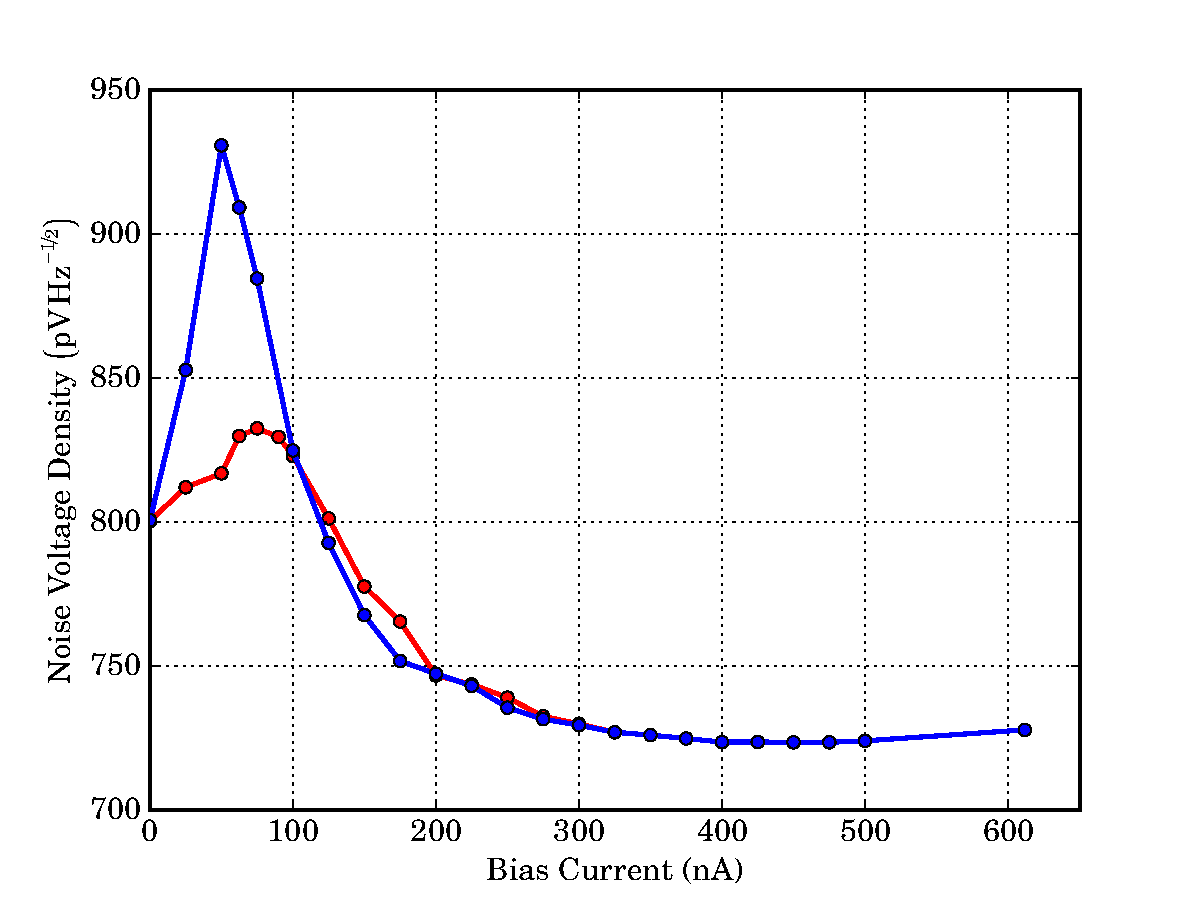
\includegraphics[width = 0.95\textwidth]{figures/strained_noiseVoltage}
\caption[Summary of the change in noise voltage with bias current for the strained-\gls{acr:SiCEB}]{Summary of the change in noise voltage with bias current for the strained-\gls{acr:SiCEB}. Blue---77-Kelvin Source; red---room-temperature source. Measured at $350~\mathrm{mK}$.}
\label{fig:strainedlNoiseV}
\end{center}
\end{figure}
All the noise spectra have been analysed by finding their average white-noise level and the results of this are shown in Figure~\ref{fig:strainedlNoiseV}. For both optical sources, the peak noise occurred slightly below the optimum bias current ($\approx\pm 90~\mathrm{nA}$). Compared to the comparable figure for the unstrained detector (Figure~\ref{fig:controlNoiseV}), not only is a greater difference seen between the two sources but also the variation in the noise voltage is also greater. 
\begin{figure}[tb]
\begin{center}
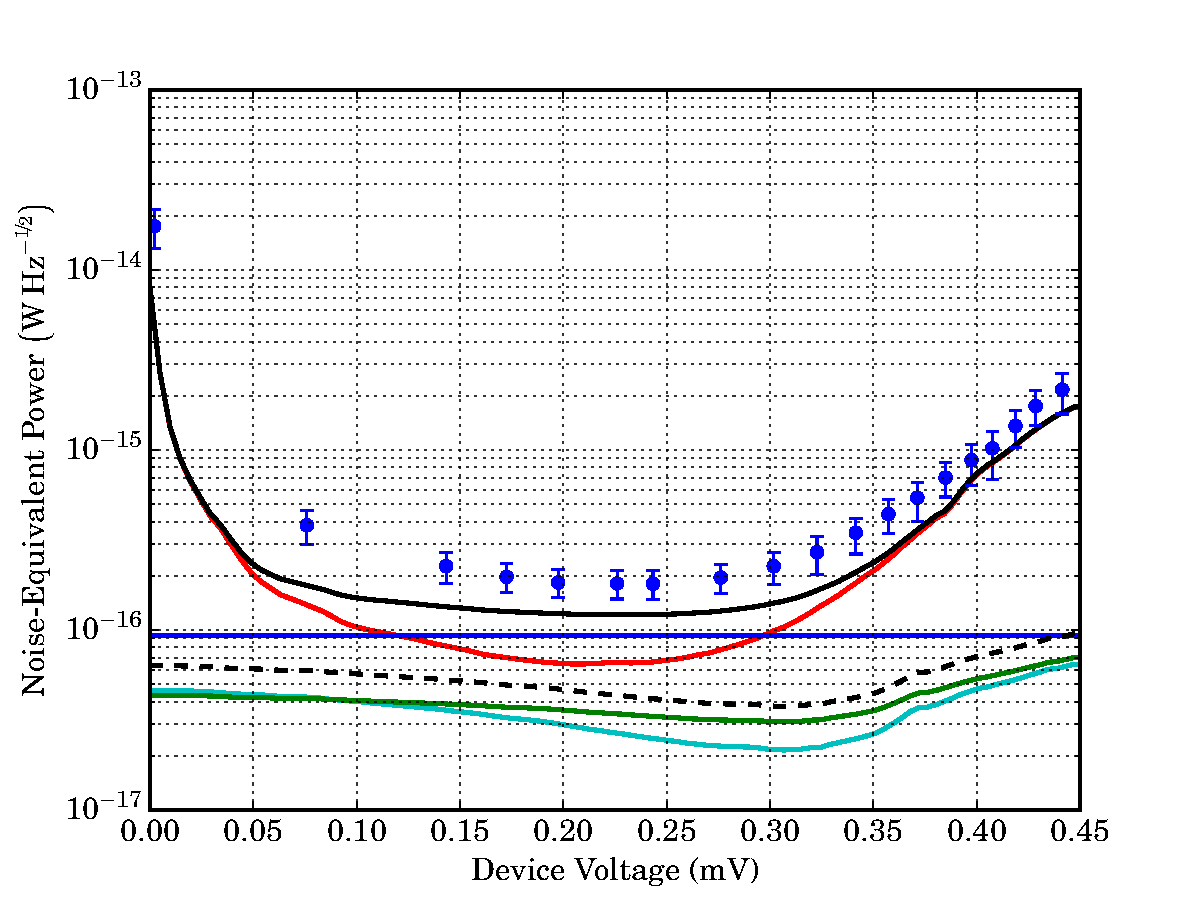
\includegraphics[width = 0.95\textwidth]{figures/strained_noiseModel300}
\caption[Noise modelling for the strained-\gls{acr:SiCEB} observing a room-temperature source]{Noise modelling for the strained-\gls{acr:SiCEB} observing a room-temperature source. Cyan---Electron-phonon heat-flow noise; green---tunnelling noise, a combination of tunnelling-current noise and the tunnelling-heat-flow noise; blue---photon noise; red---amplifier noise; black (solid)---total noise; black (dashed)---total device noise; circles---data. Measured and calculated at $350~\mathrm{mK}$.}
\label{fig:strainedNoiseModel300}
\end{center}
\end{figure}
\par
To fully explore the significance of the noise, it is necessary to model the expected contributions of the various noise sources to the final noise. Figure~\ref{fig:strainedNoiseModel300} shows the modelled noise-equivalent power, along with the measured values, for the strained detector under illumination from the room-temperature source. Firstly, unlike the comparable plot for the unstrained detector (Figure~\ref{fig:controlNoiseModel77}), it is clear that, for this detector, the amplifier noise has not dominated the measurement. Instead, the photon noise is the dominant noise source for device voltages between $0.15$ and $0.30~\mathrm{mV}$. If only the internal noise mechanisms of the detector are considered, the noise is dominated by the tunnelling noise (the final three terms in Equation~\ref{res:NEP_CEB}) and has a minimum value of $4\times 10^{-17}~\mathrm{W\,Hz^{\nicefrac{-1}{2}}}$. If all noise sources are considered, the model is close to the measured noise (circles in Figure~\ref{fig:strainedNoiseModel300}), although the error bars do not bring the two into full agreement. The model has a minimum value of $1.3\times 10^{-17}~\mathrm{W\,Hz^{\nicefrac{-1}{2}}}$, which is limited by the photon noise.
\begin{figure}[tb]
\begin{center}
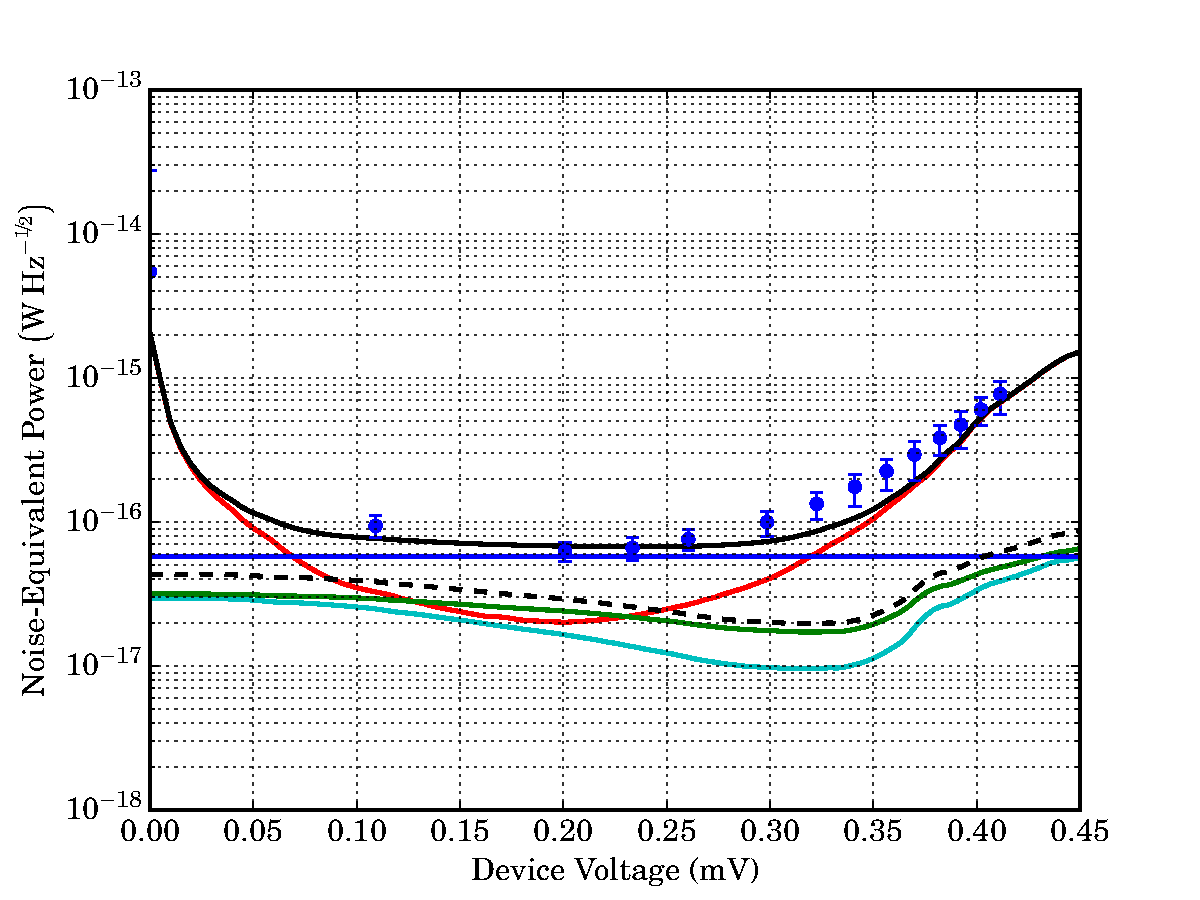
\includegraphics[width = 0.95\textwidth]{figures/strained_noiseModel77}
\caption[Noise modelling for the strained-\gls{acr:SiCEB} observing a 77-Kelvin source]{Noise modelling for the strained-\gls{acr:SiCEB} observing a 77-Kelvin source. Cyan---Electron-phonon heat-flow noise; green---tunnelling noise, a combination of tunnelling-current noise and the tunnelling-heat-flow noise; blue---photon noise; red---amplifier noise; black (solid)---total noise; black (dashed)---total device noise; circles---data. Measured and calculated at $350~\mathrm{mK}$.}
\label{fig:strainedNoiseModel77}
\end{center}
\end{figure}
\par 
Performing the same modelling, for the case where the detector was illuminated by the 77-Kelvin source, gave the model shown in Figure~\ref{fig:strainedNoiseModel77}. Here, it can be seen that the noise-equivalent power is lower overall; this is due to both the optical power being lower in this scenario and the responsivity being higher. The device-limited noise-equivalent power is still limited by the tunnelling noise, although a greater contribution from the electron-phonon noise is now seen. This is due to the electron-phonon noise not being affected by the increased responsivity, only by the slightly reduced electron temperature, whereas the tunnelling noise has decreased more substantially with the responsivity, bringing it towards the electron-phonon noise. The minimum device-limited noise-equivalent power seen in this model was $2 \times 10^{-17}~\mathrm{W\,Hz^{\nicefrac{-1}{2}}}$. Considering all noise sources (solid black line in Figure~\ref{fig:strainedNoiseModel77}), the model fits the data (circles) very well. The minimum noise-equivalent power when all noise sources were considered was $6.6 \times 10^{-17}~\mathrm{W\,Hz^{\nicefrac{-1}{2}}}$.\footnote{Note that this value differs from that reported by \textcite{Brien2014} ($1.1\times 10^{-16}~\mathrm{W\,Hz^{\nicefrac{-1}{2}}}$), where a value at device voltage of $0.32~\mathrm{mV}$ (bias current of close to $100~\mathrm{nA}$) was used. This was due to greater confidence in this point at the time of publication, due to being nearer the nominal value of $2\Delta$. However, since publication of \textcite{Brien2014}, we have gained confidence in the remainder of the data, allowing for the lower noise-equivalent power to be presented herein.} Examining the contributions to the error in the noise-equivalent power, we find that the error due the responsivity in for this measurement was $^{+1.3}_{-1.2} \times 10^{-18}~\mathrm{W\,Hz^{\nicefrac{-1}{2}}}$ from the responsivity and $\pm 9.3 \times 10^{-18}~\mathrm{W\,Hz^{\nicefrac{-1}{2}}}$ due to the measurement of the noise spectrum, thus, as was the case for the unstrained device, the measurement of the noise spectrum was the main source of error in this measurement.
\par 
Roughly speaking, one might have expected the noise-equivalent power of the strained detector to be a factor of thirty lower than the unstrained device, following the reduction in the electron-phonon coupling. However, as has been seen, the difference was nearer a factor of three. This is explained by the fact that, although the electron-phonon noise was reduced for the strained detector, this is slightly undone by the increase in the tunnelling noise (due to the higher contact resistance to the strained silicon). Overall though, the larger responsivity observed in the strained detector (which is the result of lower coupling between the electron and phonon systems) results in the noise-equivalent power being lower for the strained detector. Photon noise limited noise spectra (such as the one presented in Figure~\ref{fig:strainedNoisePlot77}) were white from the (low) \nicefrac{1}{f}-knee to the Nyquist limit ($100~\mathrm{kHz}$), showing no roll-off in the photon noise and thus indicating that the response time of this detector was $< 1.5~\mathrm{\upmu s}$.
%
\subsection{Spectral Response}\label{ssec:opticalStrainedSi_spectral}
\begin{figure}[tb]
\begin{center}
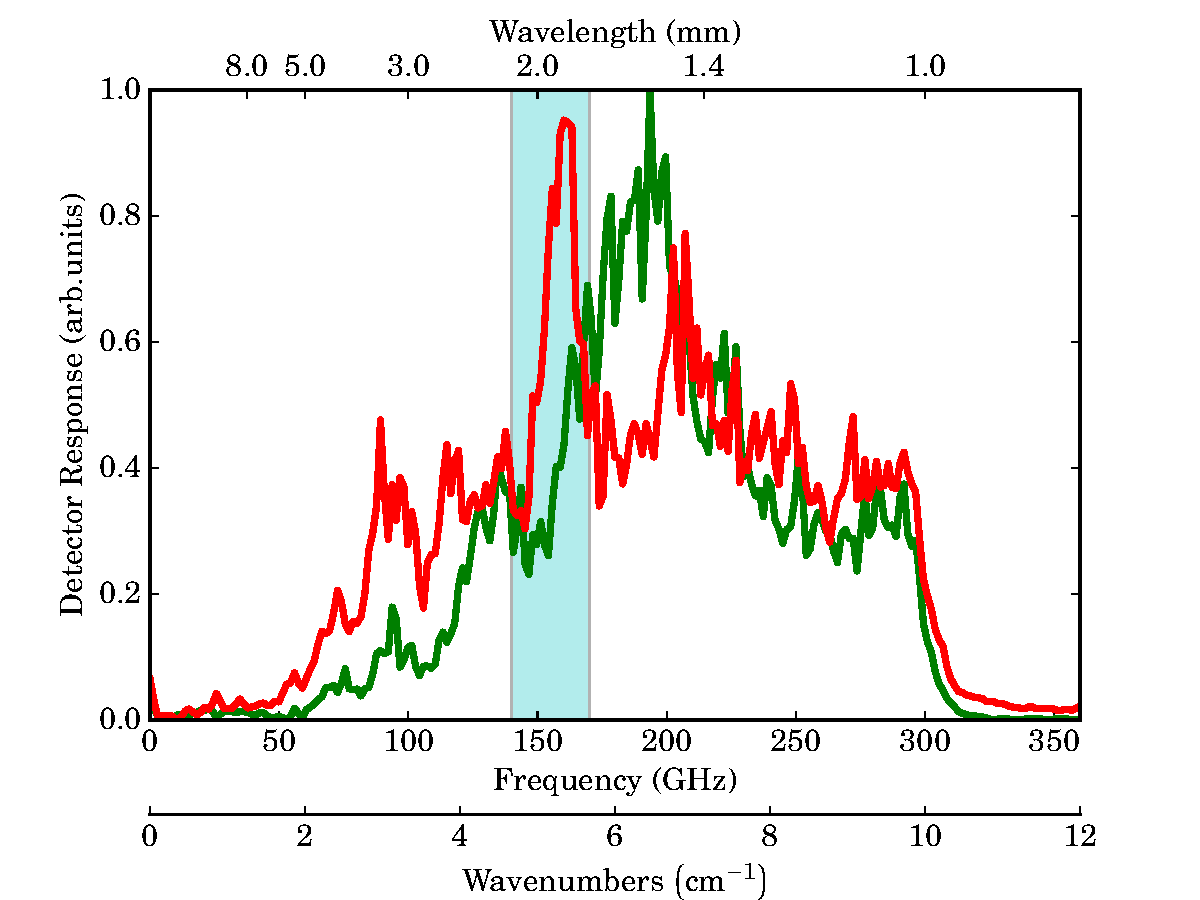
\includegraphics[width = 0.95\textwidth]{figures/strained_FTS}
\caption[Spectral response of the strained-\gls{acr:SiCEB}]{Spectral response of the strained-\gls{acr:SiCEB}, measured using a Fourier-transform spectrometer. Red---polarisation vector aligned with antenna polarisation; green---polarisation vector perpendicular to antenna polarisation; highlighted region---expected region of antenna response. In these measurements, a mercury arc lamp was used as the source. Measured at $350~\mathrm{mK}$.}
\label{fig:strainedSpectrum}
\end{center}
\end{figure}
The spectral response of the strained-silicon detector has been measured with a Fourier-transform spectrometer. A spectrum has been measured in each of the two orthogonal polarisations and the results of these measurements are shown in Figure~\ref{fig:strainedSpectrum}. There is a clear response from the detector in the polarisation aligned with that of the antenna (red plot in Figure~\ref{fig:strainedSpectrum}). There are, however, two other features in these spectra which were not anticipated. Firstly, the broad peak in the perpendicular polarisation (green plot) was not the result of the antenna response and is most likely attributed to either the coplanar waveguide and/or the DC cuts introduced into the ground plane (see Chapter~\ref{cha:Design}); or to reflections from the surfaces of the silicon lens and the device holder. The constant plateau level seen in both polarisations is most likely the result of direct absorption (i.e. not via the antenna) of optical power in the silicon mesa; it is also possible that power absorbed in the aluminium caused this. The loss of signal above $300~\mathrm{GHz}$, however, is simply due to the 300-GHz low-pass filter placed in front of the detector. The features of this spectrum will be discussed in greater detail in Section~\ref{sec:antennaSims}.
%
\subsection{Chopped-Source Measurements}\label{ssec:opticalStrainedSi_chopped}
\begin{figure}[tb]
\begin{center}
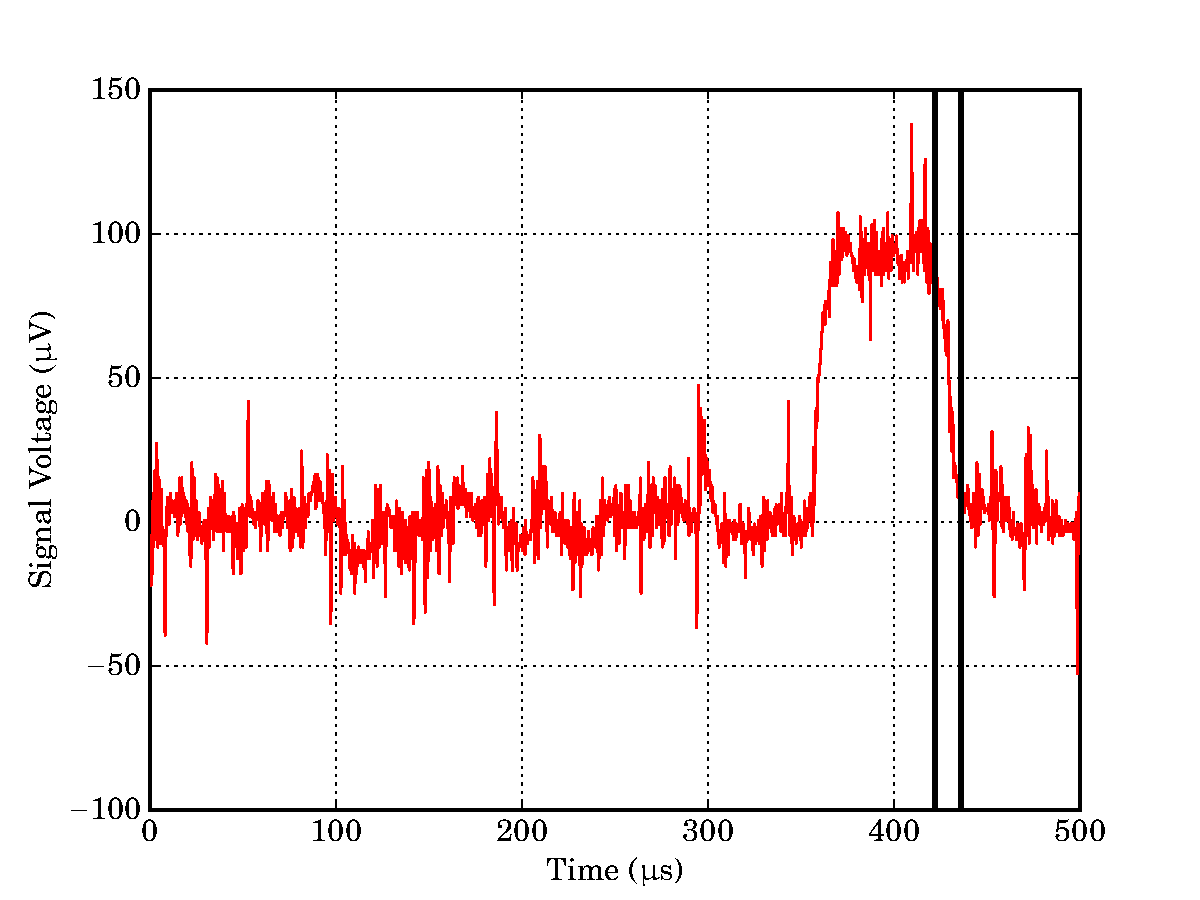
\includegraphics[width = 0.95\textwidth]{figures/strained_pulseWidth}
\caption[Time stream of the voltage signal resulting from the strained SiCEB observing a chopped signal]{Time stream of the voltage signal resulting from the strained SiCEB observing a chopped signal. The source was set to emit a pulse of $70~\mathrm{\upmu s}$, which was switched off at the first vertical black line; the voltage signal had returned to zero $14~\mathrm{\upmu s}$ later, at the second vertical black line. Measured at $280~\mathrm{mK}$.}
\label{fig:strainedChopped_time}
\end{center}
\end{figure}
In an effort to measure this detector's time constant, the response to a chopped source has been measured. The source used for this measurement was a diode (emitting radiation at $160~\mathrm{GHz}$) in a vector network analyser extender which was coupled to free space via a horn. This measurement was performed in the pulse-tube cooled system. The time stream recorded in this measurement is shown in Figure~\ref{fig:strainedChopped_time}. The source was configured to emit a $70~\mathrm{\upmu s}$ long pulse. The two vertical lines in this plot correspond to the source being switched off and the signal return to zero (the measurement was performed with a AC-coupled input). The time between the source being switched off and the signal returning to zero was measured to be $14~\mathrm{\upmu s}$. The same time has also been measured for this source using \glsfirstplural{acr:KID} and thus, it is clear that this measurement was limited by the time constant of the source as opposed to the detector. This measurement does at least allow an upper limit of $14~\mathrm{\upmu s}$ to be placed on the time constant of this detector. 
\par 
Figure~\ref{fig:strainedChopped_freq} shows a voltage spectrum measured with the detector being illuminated by the same source at a chopping frequency of $1,945~\mathrm{Hz}$. The response is immediately clear in the spectrum and has a signal-to-noise ratio of close to $1,000$.
\begin{figure}[tb]
\begin{center}
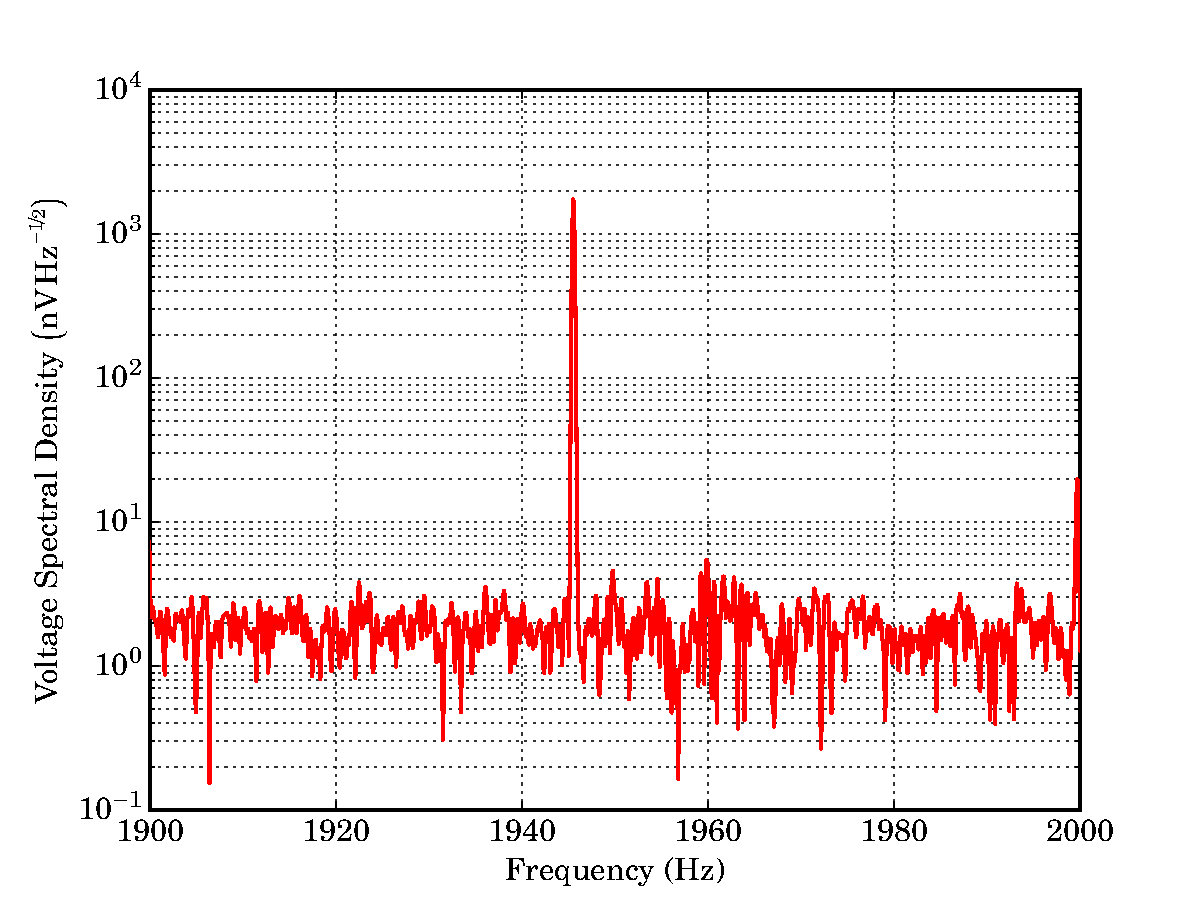
\includegraphics[width = 0.95\textwidth]{figures/strained_chopped}
\caption[Voltage spectrum measured in the presence of a 160-GHz source chopped at $1,945~\mathrm{Hz}$]{Voltage spectrum measured in the presence of a 160-GHz source chopped at $1,945~\mathrm{Hz}$. Measured at $280~\mathrm{mK}$.}
\label{fig:strainedChopped_freq}
\end{center}
\end{figure}
%
\section{Detailed Antenna Simulations}\label{sec:antennaSims}
In order to attempt to explain the spectral response of these detectors (seen earlier in this chapter) which were not as clean as had been hoped, the simulation work for the designed antenna has been revisited and expanded, in an attempt to more accurately model the detector as a whole. This section will look at the processes which have been undertaken to produce a more accurate model of the spectral response of the device. All models presented in this section have been computed using Ansys's HFSS software.\footnote{ANSYS, Inc., Southpointe, 2600 ANSYS Drive, Canonsburg, PA 15317, USA. Website: \url{http://www.ansys.com}}
%
\subsection{Basic Model: Lumped Port, Infinite Silicon}
\label{ssec:antennaSims_basic}
\begin{figure}[tb]
\begin{center}
\subfloat[]{
	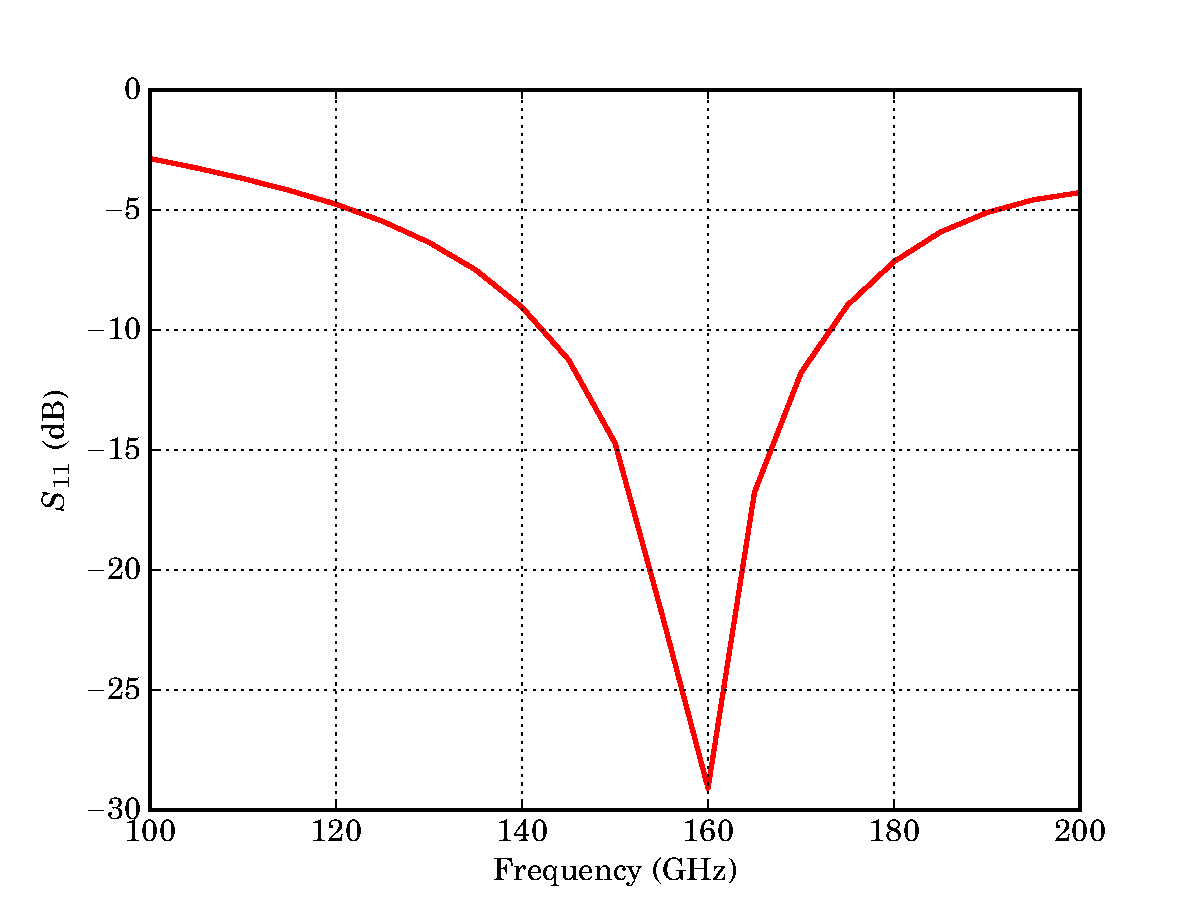
\includegraphics[width=0.5\textwidth]{figures/antennaSim_basic_S11}
	\label{fig:antennaSims_basic_S11}
}
\subfloat[]{
	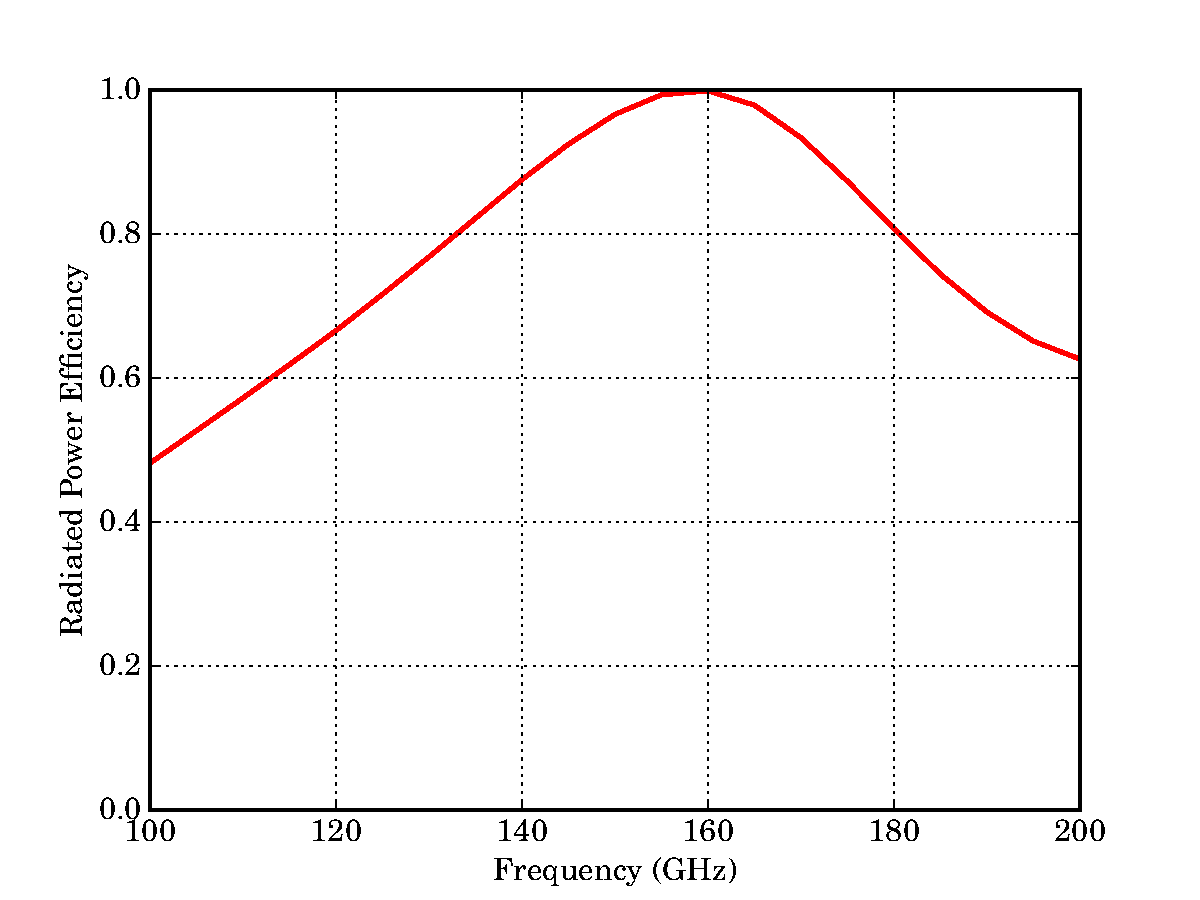
\includegraphics[width=0.5\textwidth]{figures/antennaSim_basic_Eff}
	\label{fig:antennaSims_basic_eff}
}
\caption[Initial model of the antenna, performed by measuring reflected power]{Initial model of the antenna performed by measuring reflected power from a lumped port placed at the absorber. (a) $S_{11}$ parameter; (b) radiated power efficiency.}
\label{fig:antennaSims_basic}
\end{center}
\end{figure}
The starting point for the simulation work was to revisit the initial simulation of the antenna. This rather simplistic model consisted of an emitting lumped port placed at the absorber and the reflection parameter ($S_{11}$) being calculated. The model was performed with the detector fabricated on infinitely thick silicon. The boundaries of the model were defined as reflective and placed greater than $\nicefrac{\lambda}{4}$ away from the lumped port. The absorption efficiency was also calculated using:
\begin{align}
\mathit{Eff} &= 1 - \left|S_{11}\right|^{2}\,.
\end{align}
\par 
The results of this measurement are shown in Figure~\ref{fig:antennaSims_basic}. Both the reflected power ($S_{11}$ in Figure~\ref{fig:antennaSims_basic_S11}) and the absorption efficiency (Figure~\ref{fig:antennaSims_basic_eff}) showed an excellent response at the desired frequency of $160~\mathrm{GHz}$. The 3-dB bandwidth can be seen to be ranging from approximately $100$ to $200~\mathrm{GHz}$.
\par 
From these results, it is clear that, while the initial simulation may have been incomplete, there are no fundamental issues related to the design of the antenna itself.
%
\subsection{Modelling the Antenna and Lens}\label{ssec:antennaSims_Lens}
The next step in this more detailed examination of the system was to included the silicon lens, which had not been included in the initial simulation work. The reason for using the lens was due to following similar configurations used in the measurement of hot-electron bolometers ---which are at least partly comparable to the devices tested here---and other detectors using twin-slot antennae\parencite[see for example:][along with other works by Karasik on this topic]{Ganzevles2000,Focardi2005,Karasik2011}. This silicon lens replaced the infinite silicon substrate seen in the previous model; other than this, the two models were the same and the results were computed in the same manner. In neither the model nor real life was the lens anti-reflection coated.
\begin{figure}[tb]
\begin{center}
\subfloat[]{
	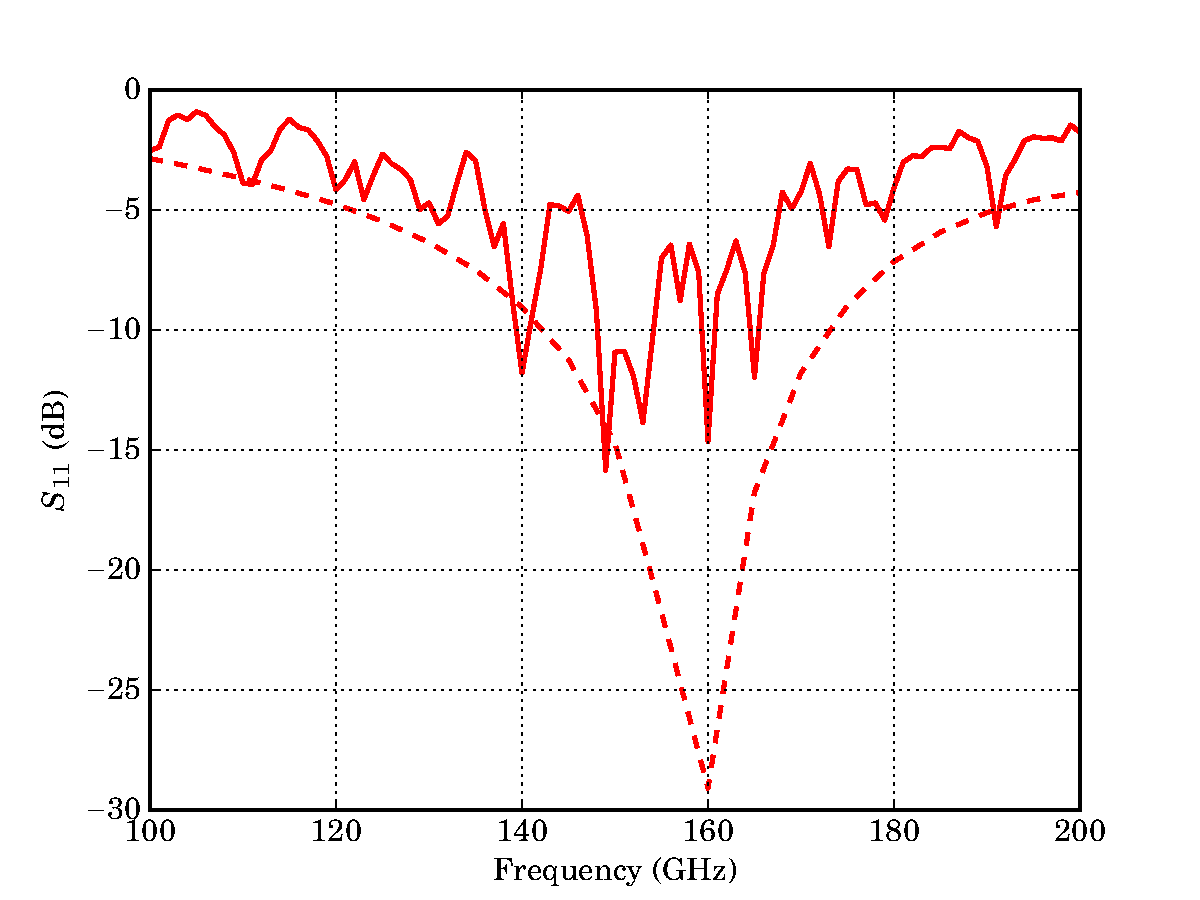
\includegraphics[width=0.5\textwidth]{figures/antennaSim_lens_S11}
	\label{fig:antennaSims_lens_S11}
}
\subfloat[]{
	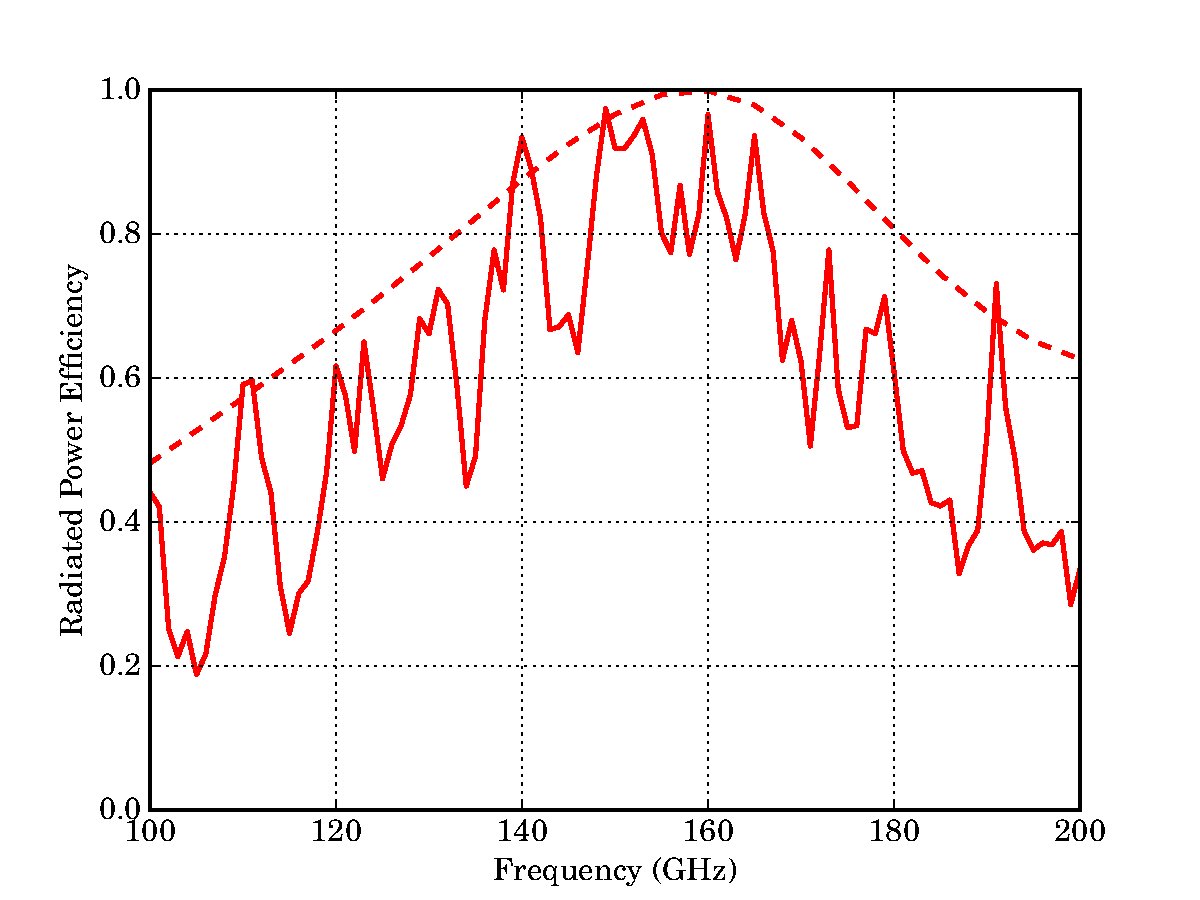
\includegraphics[width=0.5\textwidth]{figures/antennaSim_lens_Eff}
	\label{fig:antennaSims_lens_eff}
}
\caption[Model of the antenna and lens performed by measuring reflected power]{Model of the antenna and lens performed by measuring reflected power from a lumped port placed at the absorber. (a) $S_{11}$ parameter; (b) radiated power efficiency. Dashed lines---results of previous model (Figure~\ref{fig:antennaSims_basic}) for comparison.}
\label{fig:antennaSims_lens}
\end{center}
\end{figure}
\par 
The results of this revised model can be seen in Figure~\ref{fig:antennaSims_lens}. When these plots are compared to those computed for the previous model (Figure~\ref{fig:antennaSims_basic}), it is clear that the presence of the silicon lens has degraded the response of the system. In terms of the plot of the $S_{11}$ parameter (Figure~\ref{fig:antennaSims_lens_S11}), it can be seen that there is now more power reflected to the lumped port at all frequencies compared to previous model (shown as the dashed lines in Figure~\ref{fig:antennaSims_lens}). It can also be seen that the 3-dB bandwidth is reduced slightly in this case and ranges from $120$ to $170~\mathrm{GHz}$.
%
\subsection{Polarisation Model using Wave Port}\label{ssec:antennaSims_LensForw}
With the lumped-port modelling used above, it was not easily possible to measure the response of the system to the polarisation of the incoming radiation. To perform such work, the model was revised to use a wave port, placed at the input to the optical system (i.e. in front of the lens); the walls of the model were kept as reflective, as was the base of the model. The wave port was set to have two modes corresponding to the two orthogonal polarisations. In this model, the power (on a fractional basis) was modelled for each of the polarisations.
\begin{figure}[tb]
\begin{center}
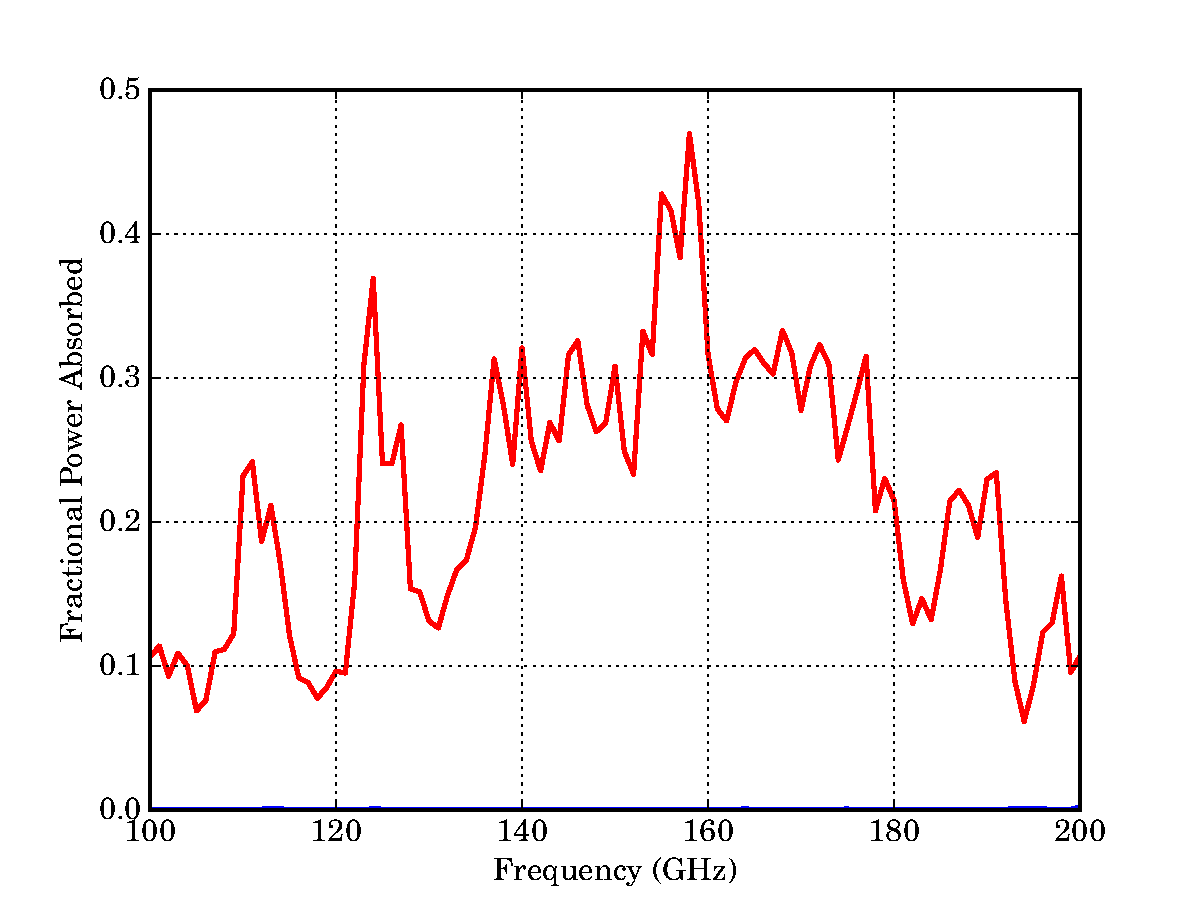
\includegraphics[width = 0.95\textwidth]{figures/antennaSim_lensForw}
\caption[Model of antenna and lens using a wave port]{Model of antenna and lens using a wave port. Red---polarisation vector aligned with that of the antenna; blue---polarisation vector perpendicular to that of the antenna}
\label{fig:antennaSims_lensForw}
\end{center}
\end{figure}
\par 
Figure~\ref{fig:antennaSims_lensForw} shows the results of this model. When the polarisation vector of the radiation emitted from the wave port is aligned with that of the antenna (red line in Figure~\ref{fig:antennaSims_lensForw}), it can be seen that power is absorbed by the silicon mesa. Although this happens over a broad range of frequencies, there is a maximum in the absorbed power just below the design frequency ($160~\mathrm{GHz}$). When the radiation's polarisation vector is perpendicular to that of the antenna (blue line Figure~\ref{fig:antennaSims_lensForw}), very little power is absorbed.
%
\subsection{Introduction of DC Cuts}\label{ssec:antennaSims_cuts}
\begin{figure}[tb]
\begin{center}
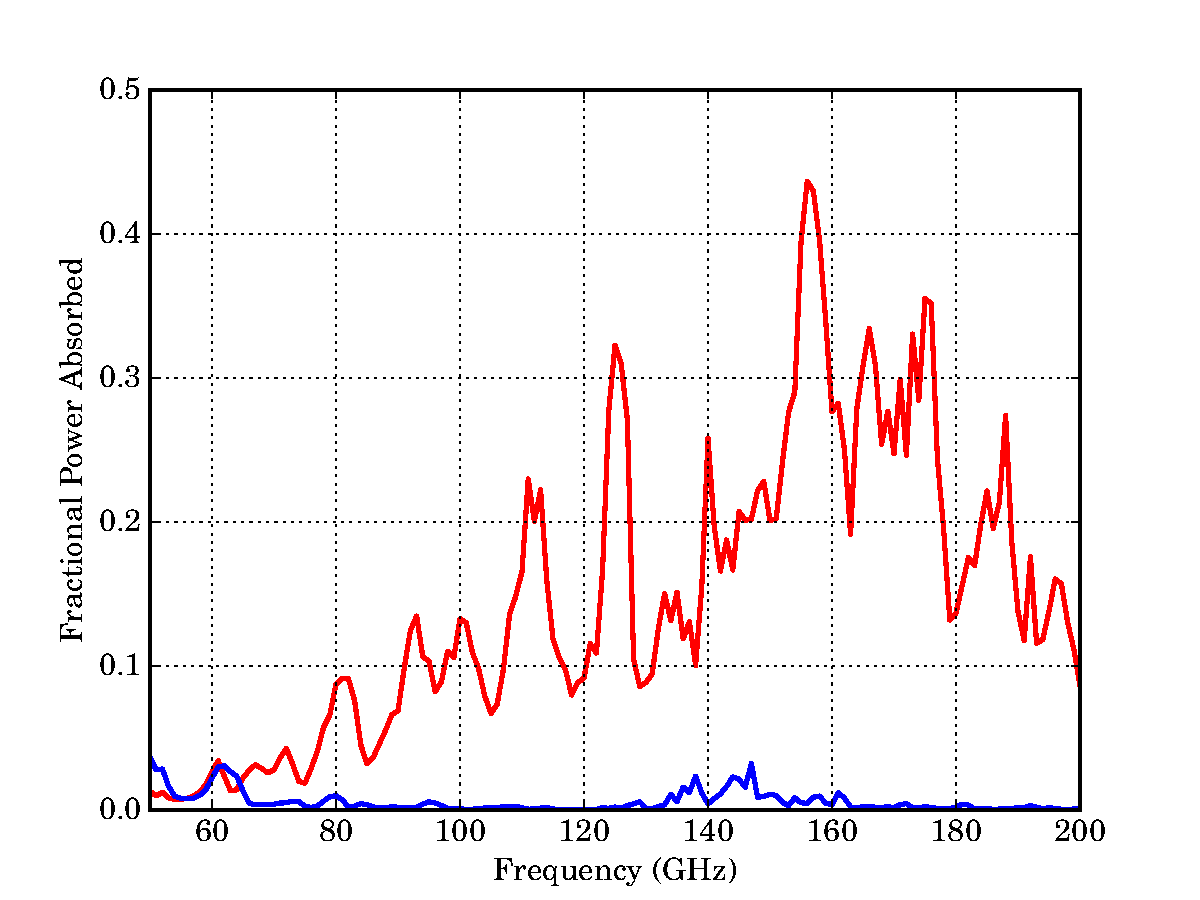
\includegraphics[width = 0.95\textwidth]{figures/antennaSim_slots}
\caption[Model of antenna, lens and DC cuts using a wave port]{Model of antenna, lens and DC cuts using a wave port. Red---polarisation vector aligned with that of the antenna; blue---polarisation vector perpendicular to that of the antenna}
\label{fig:antennaSims_slots}
\end{center}
\end{figure}
The next stage performed was to include the DC cuts in the ground plane which had not previously been modelled. This amendment was made to the model covered in the previous section and no further changes were made. The results of this model are shown in Figure~\ref{fig:antennaSims_slots}. This shows that in the aligned polarisation there is now additional absorption at $125$ and $175~\mathrm{GHz}$ but the most power is still absorbed in the silicon just below the design frequency. While there is still only a small amount of power absorbed in the perpendicular polarisation, the level is noticeably higher than in the previous model (Figure~\ref{fig:antennaSims_lensForw}). 
%
\subsection{Allowing for Loss in the Aluminium}\label{ssec:antennaSims_full}
\begin{figure}[tb]
\begin{center}
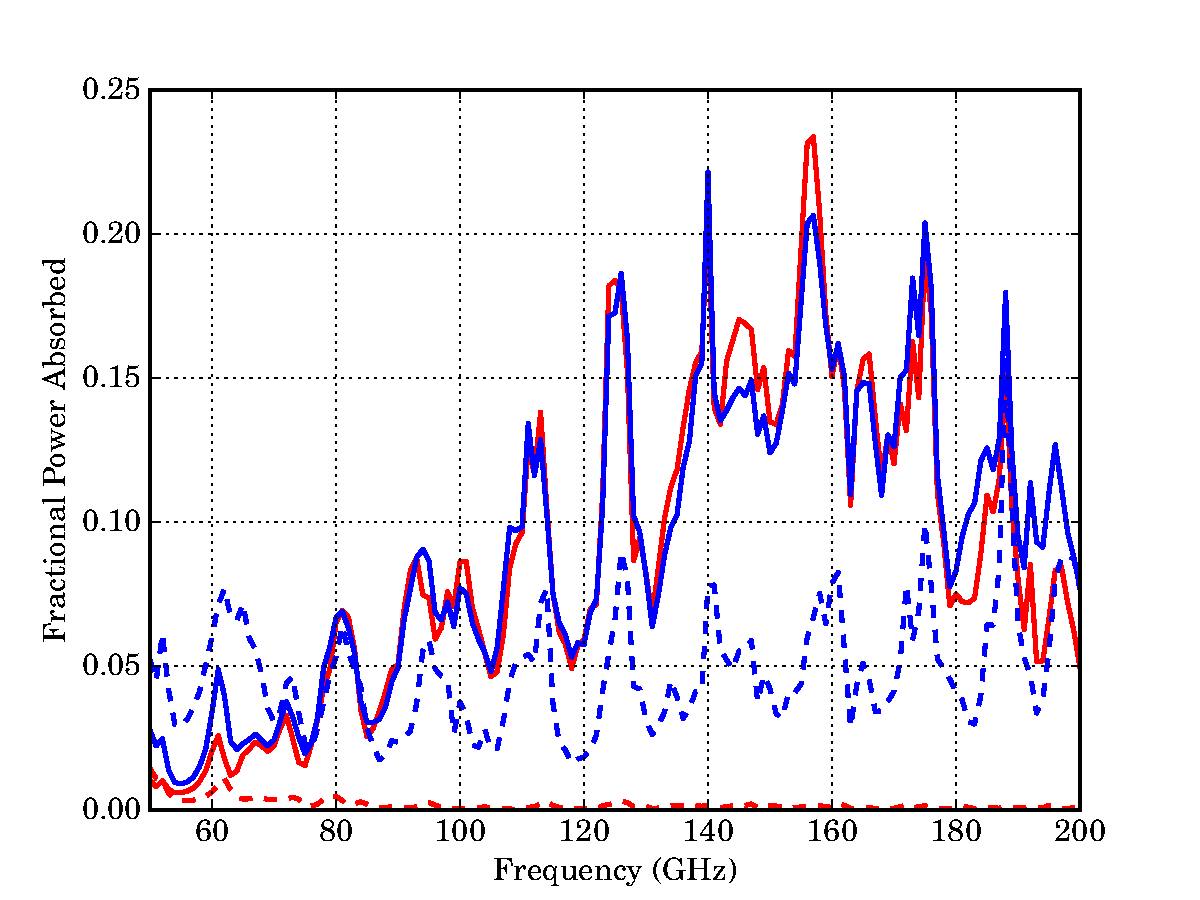
\includegraphics[width = 0.95\textwidth]{figures/antennaSim_full}
\caption[Model of antenna, lens, DC cuts and lossy aluminium using a wave port]{Model of antenna, lens, DC cuts and lossy aluminium using a wave port. Red---Absorption in the silicon mesa; blue---absorption in the aluminium; solid lines---radiation polarisation aligned with the antenna; dashed lines---radiation polarisation perpendicular to the antenna.}
\label{fig:antennaSims_full}
\end{center}
\end{figure}
The final model created was one in which the aluminium was defined to be non-perfectly conductive. This situation was intended to replicate the possible scenario whereby incoming light split Cooper pairs in the aluminium, which in turn resulted in a detector response. Clearly, in such a scenario, one would expect to see a broadband response at all frequencies above that required to split the Cooper pairs ($h\nu > 2\varDelta$). In this model, the impedance of the aluminium was set to be $1~\mathrm{\Omega/\square}$ and not only has the power absorbed in the silicon been found for polarisation but the aluminium absorption has also been modelled. The results of these measurements are shown in Figure~\ref{fig:antennaSims_full}.
\par
The results of this model (Figure~\ref{fig:antennaSims_full}) show that there is still sustainably more power absorbed when the polarisation of the incident radiation is aligned with the antenna. When the polarisations of the antenna and wave are aligned the absorption in the silicon and aluminium are comparable and the features seen in the two polarisation-aligned models seem to agree, this indicates the antenna may be coupling (losing) some power into the surrounding aluminium. When the radiation's polarisation vector is perpendicular to that of the antenna these features are also seen in the aluminium, although their magnitude is somewhat reduced. However, in the perpendicular case, very little power is absorbed within the silicon.
%
\subsection{Summary of Findings}\label{ssec:antennaSims_con}
The above simulation work has shown that, although the interpretation of the initial model of the antenna was valid and the antenna does indeed respond at the design frequency of $160~\mathrm{GHz}$, this crude model missed out several features seen when a more realistic model of the system is produced. One of the main issues raised by this work is that the silicon lens used to improve coupling of radiation to the antenna is, in fact, adversely affecting the detector response away from the design frequency. This was most likely due to the lack of an anti-reflection coating to the lens. The modelling has also shown that, should the aluminium become lossy, there would be further broadening of the response spectrum and the power absorbed in the silicon mesa would be reduced. It should be noted that the case presented in Figure~\ref{fig:antennaSims_full} is, by far, a worse-case scenario, whereby the aluminium has not only become lossy but the sheet resistance is in fact relatively high and matched to the coplanar waveguide. Clearly, from the data collected earlier in this chapter (Figures~\ref{fig:controlSpectrum} and \ref{fig:strainedSpectrum}), there is an easily distinguishable feature, due to the antenna. It is still most likely that the broadband level seen in these figures is the result of direct, bolometric, absorption by the silicon mesa, although as has been seen in this modelling work, it is possible that loss in the aluminium may have contributed to this.
%
\section{Spectral Study of Silicon Material}\label{sec:siliconFTS}
The final set of experiments performed in the course of this work were to measure the transmission properties of the silicon material as a function of frequency. The purpose of these measurements was to ascertain if the material would place any limits on the frequency range over which such a detector may be useful (i.e. capable of responding to light). Although such measurements have been carried out for bulk silicon \parencite[see for example][]{Hawkins1998}, no such measurements have been performed for highly-doped silicon  either with or without strain, such as the material used here.
\par 
This measurement was performed using the same Fourier-transform spectrometer already used to measure the spectral response of the \gls{acr:SiCEB} detectors. For these measurements, a well-characterised bolometetric detector (specifically a gold-sapphire composite bolometer operating at $1.5~\mathrm{K}$) was used to measure the signal transmitted through the material. Two samples were prepared for each of the two silicon materials (the unstrained and the strained material, both of which were highly doped). Firstly, one sample was prepared where the doped layer (along with straining layer, where relevant) was removed, this sample was used to ensure that the bulk silicon (through which the detector was illuminated) did not interfere with the measurement. Secondly, a sample of the complete wafer material was prepared; this, combined with the information already collected about the substrate, would demonstrate the affect of the doped (and strained,in the case of the second device) layer. All samples were mounted in front of the detector at a temperature of $1.5~\mathrm{K}$.
\begin{figure}[tb]
\begin{center}
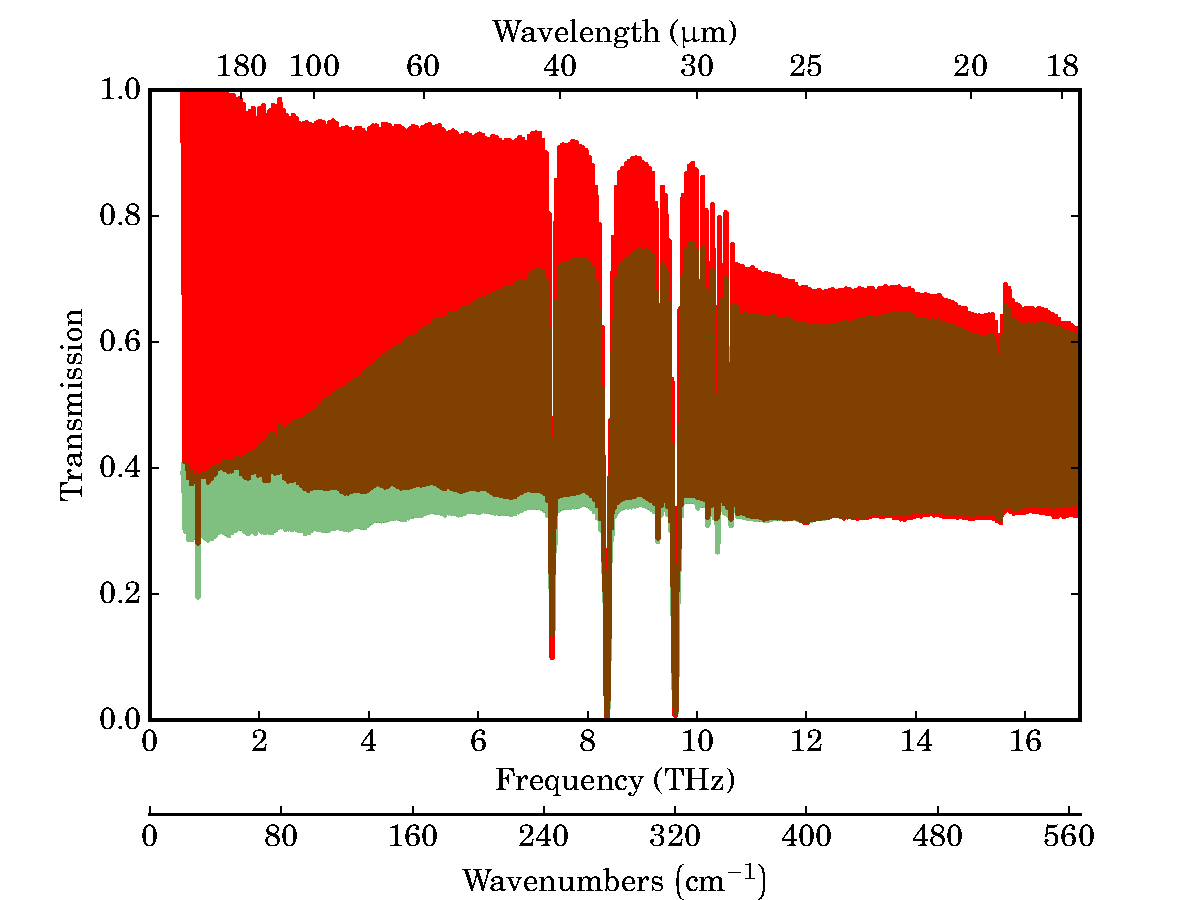
\includegraphics[width = 0.95\textwidth]{figures/control_materialFTS}
\caption[Transmission spectrum of unstrained doped silicon]{Transmission spectrum of unstrained doped silicon. Red---silicon substrate only; green---full wafer (including doped layer).}
\label{fig:control_materialFTS}
\end{center}
\end{figure}
\par
Figure~\ref{fig:control_materialFTS} shows the transmission measured for the unstrained-doped silicon (green), along with its substrate alone (red). The substrate is highly transparent from the lowest frequencies measured up to approximately $10~\mathrm{THz}$, where the transmission has dropped to $0.7$, which is maintained for the rest of the spectrum. Considering the whole wafer, there is around $60~\%$ transmission at low frequencies, then the absorption  slowly drops to $40~\%$. This small drop in the absorption should not affect a detector to the extent that it would become unusable and so it may seem reasonable to assert that this material could be used up to $17~\mathrm{THz}$ (the extent over which data have been collected).
\begin{figure}[tb]
\begin{center}
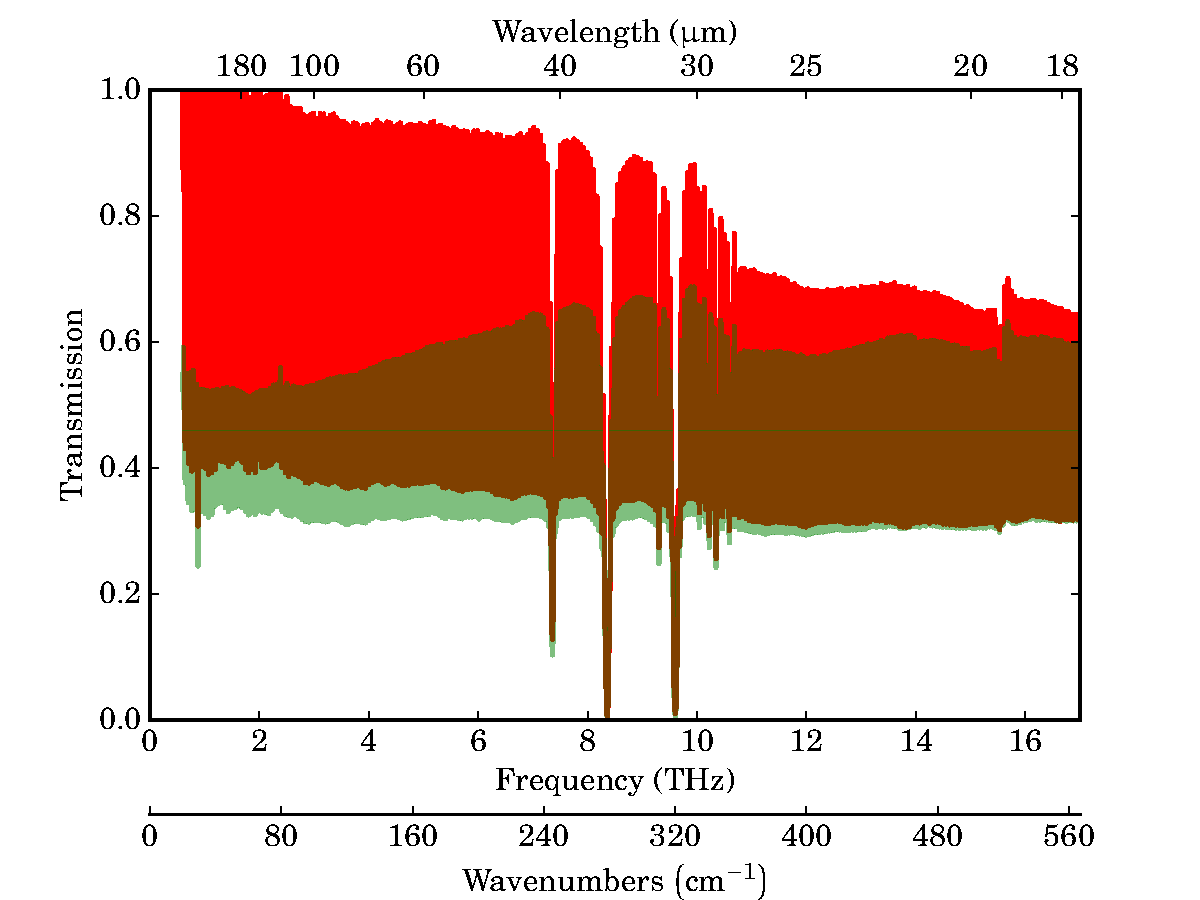
\includegraphics[width = 0.95\textwidth]{figures/strained_materialFTS}
\caption[Transmission spectrum of strained doped silicon]{Transmission spectrum of strained doped silicon. Red---silicon substrate only; green---full wafer (including doped layer).}
\label{fig:strained_materialFTS}
\end{center}
\end{figure}
\par 
Figure~\ref{fig:strained_materialFTS} shows the same spectrums measured with for the wafer with strained silicon. With the straining and doped layers removed (red plot in Figure~\ref{fig:strained_materialFTS}), the wafer transmission was, reassuringly, much the same as was seen for the previous wafer in Figure~\ref{fig:control_materialFTS}. When the strain and doped layers are considered (green plot in Figure~\ref{fig:control_materialFTS}), absorption at a level of $60~\%$ can be seen from low frequencies up to $3~\mathrm{THz}$. Above this frequency, the material becomes gradually more transmissive, until at $7~\mathrm{THz}$, where the absorption has decreased to $40~\%$, a level which is, for the most part maintained, for the remainder of the measurement. This measurement, as was the case for the unstrained material, still shows that it should be possible to use highly-doped strained silicon as an absorber up to $17~\mathrm{THz}$.\footnote{Note that this is not to say that the material would cease to be useable at $17~\mathrm{THz}$, simply that the data collected do not allow for the performance of the material above this frequency to be inferred.} It should be noted that these measurements start at a frequency of $600~\mathrm{GHz}$ compared to the operating frequency of $160~\mathrm{GHz}$ for the detectors described in this work. While not ideal, this does not present a fundamental issue with these data, since there is no reason to believe the lower-frequency behavior would change from the lowest frequencies measured (as can be seen from the mostly flat behaviour at the start of Figures~\ref{fig:control_materialFTS} and \ref{fig:strained_materialFTS}). This is further justified by the fact that the main cause for the increasing transparency of the material is the roll-off in the kinetic inductance of the carriers which, as seen from the figures in this section, occurs around $6~\mathrm{THz}$.
\par 
It should be noted that while the data contained in Figures~\ref{fig:control_materialFTS} and \ref{fig:strained_materialFTS} appear as blocks rather than lines (especially in print) they are, in fact, sinusoidal oscillations in the transmission as a result of Fabry-Perot interference due to multiple surface reflections within the sample, which can be considered to be two parallel reflecting plates. This means that the transmission, $T$, can be described by:
\begin{align}
T = \frac{\left(1-R^{2}\right)^{2}}
	{1-R^{2}\left(2\cos\left(\dfrac{4\pi nd}{\lambda}\right)\right)+R^{4}}\,,
\label{eqn:FPinterference}
\end{align}
where $R$ is the reflectance of the plates (taken to be the same for both planes), $n$ in the order, and $d$ is the distance between the two plates. For clarity Figure~\ref{fig:FTS_zoom} shows a magnified view of the data presented in this section over a much smaller frequency range. This shows the sinusoidal behaviour clearly.
\begin{figure}[tb]
\begin{center}
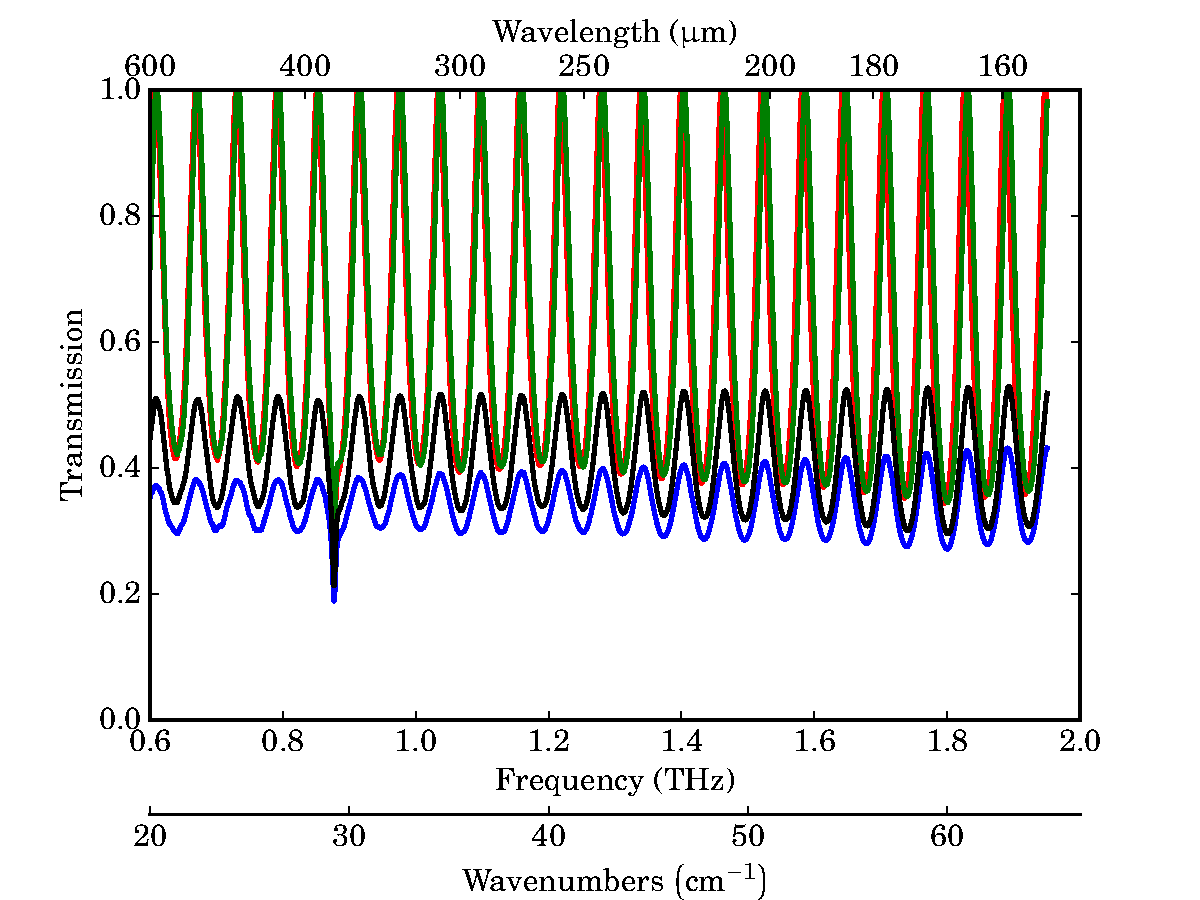
\includegraphics[width = 0.95\textwidth]{figures/Si_FTS}
\caption[Transmission of silicon material over a narrow frequency range]{Transmission of silicon material over a narrow frequency range. Fabry-Perot interference is clearly shown as the sinusoidal variations in the signal. Red---unstrained material with doped layer removed, green---strained material with doped and straining layers removed, blue---full unstrained wafer, black---full strained wafer. Measured at a temperature of $1.5~\mathrm{K}$.}
\label{fig:FTS_zoom}
\end{center}
\end{figure}
\par 
The absorption lines seen at $0.25$, $7.36$, $8.36$, and $9.60~\mathrm{THz}$ in all the measurements presented in this chapter are simply absorption lines of silicon. As are those seen between $10$ and $11~\mathrm{THz}$ \parencite{Kramida2014,Nahar1993}.
%
\section{Summary of Detector Performance}
The results in this chapter have shown that the silicon cold-electron bolometer is a sensitive detector capable of achieving sensitivities (noise-equivalent powers) of $\sim 10^{-17}~\mathrm{W\,Hz^{\nicefrac{-1}{2}}}$. These sensitivities have been achieved for a relatively unrefined, proof-of-concept-type, device. However, these sensitivities are still close to those of the detectors used in the last generation of space-based missions (see Table~\ref{tab:detectorRequirements}) and are already capable of being background limited on any ground-based instrument. To be suitable for the next generation of space based missions (for example \textit{SPICA} or \textit{SAFIR}), improvements will be required. However, as already mentioned, the devices tested throughout this work are first-generation, prototype, detectors and there is great scope for improvement. Firstly, the current absorbing element is much larger than required ($14 \times 32~\mathrm{\upmu m}$), reducing the size of this element would lower the noise-equivalent power associated with the interaction between the electron and phonon systems (Equation~\ref{eqn:NEP_e-ph}). Calculations performed for a comparable device, where the absorber is reduced in size by a factor of ten, give $NEP_{\mathrm{e\mbox{-}ph}} = 2.6 \times 10^{-18}~\mathrm{W\,Hz^{\nicefrac{-1}{2}}}$. This shrinking is easily attainable with standard photolithography and, if e-beam lithography were to be used, further order-of-magnitude reductions could be made. Furthermore, it should be possible to further increase the strain in the absorbing layer and, as has been seen in this chapter, such a change should further reduce the interaction between the electrons and the phonons. Finally, the current tunnelling contacts could be improved to create more consistent Schottky contacts; greater control over this would allow the tunnelling noise to be lowered.

